\documentclass[nogrid]{MBE}%

\usepackage{epstopdf}

\usepackage{url}

\jshort{mst}

\volname{}

\jvolume{0}

\jvol{}

\jissue{0}

\pubyear{2013}

\mstype{Article}

\artid{012}

\access{Advance Access publication March 3, 2013}


\begin{document}

\title[Going to Extremes]{Going to Extremes:
Contrasting Rates of Diversification in a Recent Radiation of New World Passerine Birds}


\author[Barker et al.]{F. Keith \surname{Barker},$^{\ast,1,2}$ Kevin J.
Burns,$^{3}$ John Klicka,$^{4}$ Scott M. Lanyon,$^{1}$ and Irby J.~Lovette$^{5}$}

\address{$^{1}$Department of Ecology, Evolution and Behavior\\
$^{2}$Bell Museum of Natural History, University of Minnesota, 100 Ecology, 1987 Upper Buford
Circle, St Paul, MN 55108\\ $^{3}$Department of Biology, San Diego State University, San Diego, CA
92182\\ $^{4}$Marjorie Barrick Museum of Natural History, Box 454012, University of Nevada, Las
Vegas, 4505 Maryland Parkway, Las Vegas, NV 89154\\ $^{5}$Fuller Evolutionary Biology Program,
Cornell Lab of Ornithology, 159 Sapsucker Woods Road, Ithaca, NY 14850, USA}


\history{Received 13 July 2011; reviews returned 26 November 2012; accepted 30 November 2012}

\coresp{E-mail: barke042@umn.edu.}

\datade{The POPRES data were obtained from dbGaP (accession no. phs000145.v1.p1).}


\editor{Robb Brumfield}

\abstract{Recent analyses suggest that a few major shifts in diversification rate may be enough to
explain most of the disparity in diversity among vertebrate lineages. At least one significant
increase in diversification rate appears to have occurred within the birds; however, several
nested lineages within birds have been identified as hyperdiverse by different studies. A clade
containing the finches and relatives (within the avian order Passeriformes), including a large
radiation endemic to the New World that comprises $\sim $8{\%} of all bird species, may be the
true driver of this rate increase. Understanding the patterns and processes of diversification of
this diverse lineage may go a long way toward explaining the apparently rapid diversification
rates of both passerines and of birds as a whole. %We present the first multilocus phylogenetic
%analyses of this endemic New World radiation of finch relatives a relaxed molecular clock analysis
%of its divergence history, and an analysis of its broad-scale that include sampling of all
%recognized genera, a relaxed molecular clock analysis of its divergence history, and an analysis
%of its broad-scale diversification patterns. These analyses recovered 5 major lineages
%traditionally recognized as avian families, but identified an additional 10 relatively ancient
%lineages worthy of recognition at the family level. Time-calibrated diversification analyses
%suggested that at least 3 of the 15 family-level, Thraupidae---appeared significantly more
%diverse. Lack of an age--diversity relationship within this clade suggests that, due to rapid
%initial speciation, it may have experienced density-dependent ecological limits on its overall
%diversity.
}

\keyword{Concatenation, concordance, congruence, diversification, gene tree, New World,
Passeriformes.}

\maketitle



\section{{Introduction}\label{sec:Intro}}


This paper considers an overlapping generations model without external effects or a social
security system. Nonetheless, we show that a population decline can worsen the welfare of agents
if it is caused by a change in the timing of childbirth or, more specifically, when many people
decide to delay childbearing to older ages.

Delayed childbearing has been broadly observed in developed countries. Between 1975 and 2005, the
fraction of Japanese children who were born to mothers in their 20s  decreased from 75\% to 45\%,
whereas those born to mothers in their 30s increased from 20\% to 52\%. A similar trend is
observed in the United States and advanced European {countries\vvp{} (Gustafsson and Kalwij,
2006), and also in Canada, Australia, and New Zealand \citet{Hampel:1974}. Interestingly, as
pointed out by \citep{Efron:1979,Felsenstein:1985}, even when the cohort's lifetime fertility rate
(the number of children a mother has in her lifetime) does not fall, the delayed childbearing
alone leads to a decline in the number of childbirths, measured by the total period fertility
rates (TPFRs). \citet{Huber:2004}, \citet{Miller:1974}, and Sobotka (2004) confirmed that, to a
certain extent, the delay of marriage and motherhood is responsible for the observed period
fertility rate decline (now known as the `tempo effect'). This paper considers an overlapping
generations model
without external effects or a social security system. %Nonetheless, we show that a population
%decline can worsen the welfare of agents if it is caused by a change in the timing of childbirth
%or, more specifically, when many people decide to delay childbearing to older ages.

As the variation in the age composition of workers affects the distribution of income among
different cohorts (Berger, 1989), demographic cycles lead to cycles in the aggregate saving rate,
which drive fluctuations in the capital--labor ratio. We will show that the fluctuations in the
capital--labor ratio have differential  effective labor produces a fixed welfare effects on agents
depending on their positions in the demographic cycles. This point was not found by earlier
studies. For instance, \citet{Archibald_Roger:2002} considered a small open economy with a fixed
capital--labor ratio, savings were not allowed in \citet{Blouin_Butt_Roger:2005}, and
\citep{Bar-Hen_Kishino:2000} and d'Albis et al. (2010) assumed a linear technology where one unit
of effective labor produces a fixed amount of output. The remainder of the paper is structured as
follows. Section \ref{sec:Model} introduces the theoretical model. Section \ref{sec:Dyn}
analytically examines the impact of delayed childbearing on capital accumulation and welfare.
Section \ref{sec:Numerical} numerically examines the general case where only a fraction of agents
delay their childbearing. Section \ref{sec:Robustness} considers extensions of the model with a
lower lifetime fertility rate and technological progress. Section \ref{sec:Conclusion} concludes
the paper. Appendices A and B provide the proofs of the lemmas.

Delayed childbearing has been broadly observed in developed countries. Between 1975 and 2005, the
fraction of Japanese children who were born to mothers in their 20s decreased from 75\% to 45\%,
whereas those born to mothers in their 30s increased from 20\% to 52\%. A similar trend is
observed in the United States and advanced European countries \citet{Bryant_Galtier_Poursat:2005},
and
also in Canada, Australia, and New Zealand \citep{Efron:1979}. %Interestingly, as pointed out by
%Bongaarts and Feeney (1998), even when the cohort's lifetime fertility rate (the number of
%children a mother has in her lifetime) does not fall, the delayed childbearing alone leads to a
%decline in the number of childbirths, measured by the total period fertility rates (TPFRs). Ogawa
%and Retherford (1993), Kohler et al. (2002), and Sobotka (2004) confirmed that, to a certain
%extent, the delay of marriage and motherhood is responsible for the observed period fertility rate
%decline (now known as the `tempo effect').This paper considers an overlapping generations model
%without external effects or a social security system. Nonetheless, we show that a population
%decline can worsen the welfare of agents if it is caused by a change in the timing of childbirth
%or, more specifically, when many people decide to delay childbearing to older ages.



\section{Demographic structure}

Delayed childbearing has been broadly observed in developed countries. Between 1975 and 2005, the
fraction of Japanese children who were born to mothers in their 20s decreased from 75\% to 45\%,
whereas those born to mothers in their 30s increased from 20\% to 52\%. A similar trend is
observed in the United States and advanced European countries (Gustafsson and Kalwij, 2006), and
also in Canada, Australia, and New Zealand \citep{Efron:1979}.

\subsection{Demographic structure}

Interestingly, as pointed out by \citep{Miller:1974,Efron:1979}, even when the cohort's lifetime
fertility rate (the number of children a mother has in her lifetime) does not fall, the delayed
childbearing alone leads to a decline in the number of childbirths, measured by the total period
fertility rates (TPFRs).

\subsubsection{Demographic structure}
Ogawa and Retherford (1993), Kohler et al. (2002), and \citep{Miller:1974} confirmed that, to a
certain extent, the delay of marriage and motherhood is responsible for the observed period
fertility rate decline (now known as the `tempo effect').This paper considers an overlapping
generations model without external effects or a social security system. Nonetheless, we show that
a population decline can worsen the welfare of agents if it is caused by a change in the timing of
childbirth or, more specifically, when many people decide to delay childbearing to older ages.
Iyigun (2000) built a growth model where women face a tradeoff between childbearing and human
capital accumulation when young, and derived multiple steady state equilibria.
\citet{Vandenkoornhuyse_Baldauf_Leyval_Straczek_Young:2002} illustrated the mechanism where an
increase in longevity delays the timing of childbearing. \citet{Guindon_Gascuel:2003} constructed
an endogenous childbirth timing model where the solution is obtained as a closed form. d'Albis et
al.\ (2010) proved the existence of a monetary equilibrium in a model where the age of
childbearing is determined endogenously.
%
%
%Delayed childbearing has been broadly observed in developed countries. Between 1975 and 2005, the
%fraction of Japanese children who were born to mothers in their 20s decreased from 75\% to 45\%,
%whereas those born to mothers in their 30s increased from 20\% to 52\%. A similar trend is
%observed in the United States and advanced European countries (Gustafsson and Kalwij, 2006), and
%also in Canada, Australia, and New Zealand (Sardon, 2006). Interestingly, as pointed out by
%Bongaarts and Feeney (1998), even when the cohort's lifetime fertility rate (the number of
%children a mother has in her lifetime) does not fall, the delayed childbearing alone leads to a
%decline in the number of childbirths, measured by the total period fertility rates (TPFRs). Ogawa
%and Retherford (1993), Kohler et al. (2002), and Sobotka (2004) confirmed that, to a certain
%extent, the delay of marriage and motherhood is responsible for the observed period fertility rate
%decline (now known as the `tempo effect').
%



\paragraph{Demographic structure.} Of course, the declining birth rate can cause welfare problems when the
population size has some positive externality, or when social security systems are explicitly
considered. {To support a pay-as-you-go pension system, the economy must have enough children.}
Apart from these issues, it has been generally perceived that the population decline is favorable
to economic welfare. {A notable exception is \citep{Felsenstein:2004}, which showed that when
agents are uncertain about the length of their life and there is a perfect annuity market, the
capital--labor ratio may respond nonmonotonically to the population growth rate.}



This paper considers an overlapping generations model without external effects
or a social security system. Nonetheless, we show that a population decline
can worsen the welfare of agents if it is caused by a change in the timing of
childbirth or, more specifically, when many people decide to delay
childbearing to older ages.

%This paper considers an overlapping generations model without external effects or a social
%security system. Nonetheless, we show that a population decline can worsen the welfare of agents
%if it is caused by a change in the timing of childbirth or, more specifically, when many people
%decide to delay childbearing to older ages.

 As the variation in the age composition of workers affects
the distribution of income among different cohorts \citep{Posada_Crandall:1998}, demographic
cycles lead to cycles in the aggregate saving rate, which drive fluctuations in the capital--labor
ratio. We will show that the fluctuations in the capital--labor ratio have differential welfare
effects on agents depending on their positions in the demographic cycles. This point was not found
by earlier studies. For instance, Iyigun (2000) considered a small open economy with a fixed
capital--labor ratio, savings were not allowed in \citep{Posada_Crandall:1998}, and Mullin and
Wang (2002) and d'Albis et al. (2010) assumed a linear technology where one unit of effective
labor produces a fixed amount of output. The remainder of the paper is structured as follows.
Section \ref{sec:Model} introduces the theoretical model. Section \ref{sec:Dyn} analytically
examines the impact of delayed childbearing on capital accumulation and welfare. Section
\ref{sec:Numerical} numerically examines the general case where only a fraction of agents delay
their childbearing. Section \ref{sec:Robustness} considers extensions of the model with a lower
lifetime fertility rate and technological progress. Section \ref{sec:Conclusion} concludes the
paper. Appendices A and B provide the proofs of the lemmas.

Delayed childbearing has been broadly observed in developed countries. Between 1975 and 2005, the
fraction of Japanese children who were born to mothers in their 20s decreased from 75\% to 45\%,
whereas those born to mothers in their 30s increased from 20\% to 52\%. A similar trend is
observed in the United States and advanced European countries (Gustafsson and Kalwij, 2006), and
also in Canada, Australia, and New Zealand
\citet{Vandenkoornhuyse_Baldauf_Leyval_Straczek_Young:2002}. Interestingly, as pointed out by
Bongaarts and Feeney (1998), even when the cohort's lifetime fertility rate (the number of
children a mother has in her lifetime) does not fall, the delayed childbearing alone leads to a
decline in the number of childbirths, measured by the total period fertility rates (TPFRs). Ogawa
and Retherford (1993), Kohler et al. (2002), and Sobotka (2004) confirmed that, to a certain
extent, the delay of marriage and motherhood is responsible for the observed period fertility rate
decline (now known as the `tempo effect').This paper considers an overlapping generations model
without external effects or a social security system. Nonetheless, we show that a population
decline can worsen the welfare of agents if it is caused by a change in the timing of childbirth
or, more specifically, when many people decide to delay childbearing to older ages.


The seminal studies that incorporated the tempo effect into economic theory are Happel et al.\
(1984) and \citep{Zucker_Mathews_Turner:1999}. These studies constructed models where women
endogenously choose their career paths or the accumulation of human capital. {For empirical
studies on this issue, see \citep{Penny_Hendy:1985}, which employed the National Longitudinal
Survey of Youth to investigate the return to delayed childbearing in the US. Using Japanese panel
data, Higuchi (2001) investigated the effects of labor market changes on the timing of marriage,
childbirth, and employment.} Incorporating this idea into the theory of economic growth, Iyigun
(2000), \citet{Huber:2004}, Mullin and Wang (2002), and d'Albis et al.\ (2010) constructed dynamic
general equilibrium models where
the timing of childbirth is endogenous.%\footnote{Iyigun (2000) built a growth
%model where women face a tradeoff between childbearing and human capital
%accumulation when young, and derived multiple steady state equilibria.
%Blackburn and Cipriani (2002) illustrated the mechanism where an increase in
%longevity delays the timing of childbearing. Mullin and Wang (2002)
%constructed an endogenous childbirth timing model where the solution is
%obtained as a closed form. d'Albis et al.\ (2010) proved the existence of a
%monetary equilibrium in a model where the age of childbearing is determined
%endogenously.}
\begin{arabiclist}
\item Consider a fall in population induced by a decline in the number of births in the economy,
taking as given mortality and migration.

\item It is well known that a lower population growth raises the capital--labor ratio in the Solow--Swan
growth model.

\item The same property holds in Diamond's (1965) overlapping generations model, and it enhances welfare
as long as the economy is dynamically efficient; i.e., when the interest rate exceeds the
population growth rate.
\end{arabiclist}
Complementary to these preceding studies, this paper focuses on the aspect that delayed
childbearing changes the age structure of the labor force. When a considerable fraction of mothers
begin to delay childbearing, it causes a temporary baby bust in the economy, and the echoes of the
initial baby bust create long-lasting demographic cycles. %We construct an overlapping generations
%model where agents work for more than one period so that the demographic cycles are translated
%into fluctuations in the age structure of the labor force.
\begin{itemize}
\item Consider a fall in population induced by a decline in the number of births in the economy,
taking as given mortality and migration.

\item It is well known that a lower population growth raises the capital--labor ratio in the Solow--Swan
growth model.

\item The same property holds in Diamond's (1965) overlapping generations model, and it enhances welfare
as long as the economy is dynamically efficient; i.e., when the interest rate exceeds the
population growth rate.
\end{itemize}
 A similar trend is observed in the United
States and advanced European countries (Gustafsson and Kalwij, 2006), and also in Canada,
Australia, and New Zealand (Sardon, 2006). Interestingly, as pointed out by Bongaarts and Feeney
(1998), even when the cohort's lifetime fertility rate (the number of children a mother has in her
lifetime) does not fall, the delayed childbearing alone leads to a decline in the number of
childbirths, measured by the total period fertility rates (TPFRs). %Ogawa and Retherford (1993),
%Kohler et al. (2002), and Sobotka (2004) confirmed that, to a certain extent, the delay of
%marriage and motherhood is responsible for the observed period fertility rate decline (now known
%as the `tempo effect').


\section{Model\label{sec:Model}}

\subsection{Demographic structure}



Let us consider an overlapping generations model where each agent lives for
four periods, referred to as child, young, middle-aged, and old. A group of
young agents in period $t$ (i.e., those who are born in period $t-1$) is
called generation $t$, and its cohort size is denoted by $N_{t}$. Each agent
has one child during her lifetime (the gender of the agents is not
considered), and she is able to bear a child either in her youth or middle
age. In this paper, we say that an agent `delays childbearing'\ if she bears
her (only) child in her middle age.

\subsubsection{Demographic structure}

Let us denote by $\lambda_{t}\in\left[  0,1\right]  $ the fraction of agents
among generation-$t$ agents who delay childbearing. This means that among the
generation-$t$ agents with population $N_{t}$, the fraction $\lambda_{t}$ bear
their children in their middle age (period $t+1$), and the remaining fraction
$1-\lambda_{t}$ bear their children in their youth (period $t$). The cohort
size of generation $t+1$, born in period $t$, is thus determined by:%
\begin{equation}
N_{t+1}=\left(  1-\lambda_{t}\right)  N_{t}+\lambda_{t-1}N_{t-1}.
\label{eq:PopDyn}%
\end{equation}


To highlight the effect of age distribution on capital accumulation and welfare as simply as
possible, the timing of childbearing is assumed to be exogenous throughout the analysis. {Doepke
(2005) showed that the timing of childbirth is affected by the child mortality rate in a
sequential fertility choice model. A decline in child mortality also reduces the uncertainty about
the number of surviving children, which lowers the fertility rate and raises educational
investment, causing the demographic transition (Kalemli-Ozcan, 2002, 2003; Tamura, 2006).} We
consider the situation where all agents until generation $-1$ bear their children when they are
young, and from generation 0 a constant fraction $\lambda$ of agents bear their children when they
are middle-aged, i.e.:
\begin{equation}
\lambda_{t}=\left\{
\begin{array}
[c]{cc}%
0, & t<0,\\
\lambda, & t\geq0.
\end{array}
\right.  \label{eq:lambda}%
\end{equation}


We normalize the cohort size so that $N_{0}=1$ holds. As equations
(\ref{eq:PopDyn}) and (\ref{eq:lambda}) imply that the cohort size is constant
until period 0, $N_{t}=1$ holds for all $t\leq0$. When delayed childbearing
begins, the period fertility rate temporarily falls. In period 0, only
fraction $1-\lambda$ of generation-0 young agents bear children, while the
generation-($-1$) middle-aged agents do not bear children because they
completed childbearing in the previous period (i.e., $\lambda_{-1}=0$). Thus,
the cohort size of generation 1, who are born in period 0, is given by:
\begin{equation}
N_{1}=1-\lambda. \label{eq:N1}%
\end{equation}


\begin{figure}[t]
\begin{center}
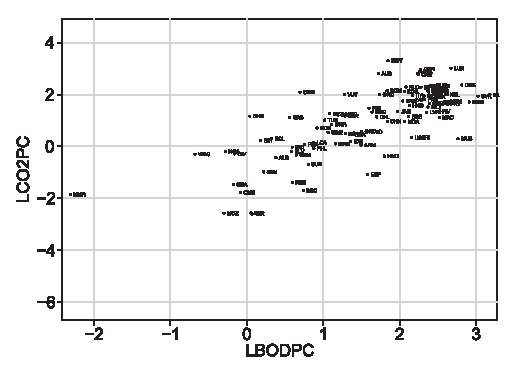
\includegraphics{flrf1.eps}
\end{center}
\caption{Fluctuations in Cohort Size $N_{t}$ over Generations.}%
\label{fig:popdynamics}%
\end{figure}

%\TWOfig{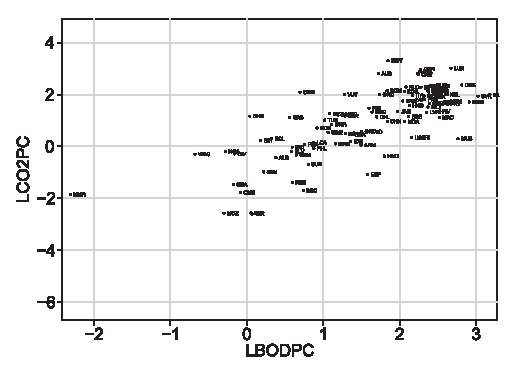
\includegraphics[width=10pc]{flrf1.eps}}{Fluctuations in
%Cohort Size $N_{t}$ over
%Generations.\label{fig:popdynamics}}{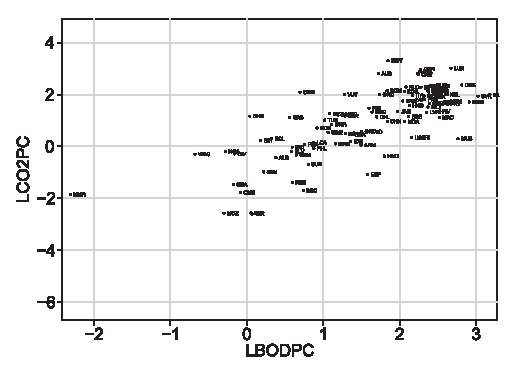
\includegraphics[width=10pc]{flrf1.eps}}{Dynamics
%of Labor Force $L_{t}$.\newline
%\phantom{\hskip5pc}\label{fig:labordynamics}}

From period $1$ on, not only a fraction $1-\lambda$ of young agents, but also a fraction $\lambda$
of middle-aged agents bear children. Hence, the period fertility rate recovers to some extent,
which is consistent with Bongaarts and Feeney (1998). Substituting $N_{0}=1$, $N_{1}=1-\lambda$,
and equation (\ref{eq:lambda}) into (\ref{eq:PopDyn}), the cohort size after generation 0 is
solved as $N_{t}=\frac{1}{1+\lambda}\left(  1+\left(  -1\right) ^{t}\lambda^{t+1}\right)  $ for
$t\geq0$. Figure~1 depicts the sequences of $N_{t}$ for various levels of $\lambda$. It shows that
the cohort size $N_{t}$ fluctuates after delayed childbearing begins (i.e., after period 0), and
that the amplitude of oscillation is larger when $\lambda$ is higher. This indicates that the
initial fluctuation of age structure (i.e., the fall in the fertility rate in period 0 and a
recovery in period 1) has recurrent `echo effects' over many generations. If $\lambda\in\left(
0,1\right)  $, the fluctuation decays and $N_{t}$ converges to a stationary level at
$\lim_{t\rightarrow\infty}N_{t}={1}/({1+\lambda})$, {This is consistent with Lotka's stable
population theory, which states that in a closed economy where there is no migration, a long-run
age distribution becomes time invariant when age-specific fertility and mortality rates are
constant (see Keyfitz and Caswell, 2005).} although $N_{t}$ fluctuates forever in the polar case
of $\lambda=1$.

\begin{figure*}[t]
\begin{center}
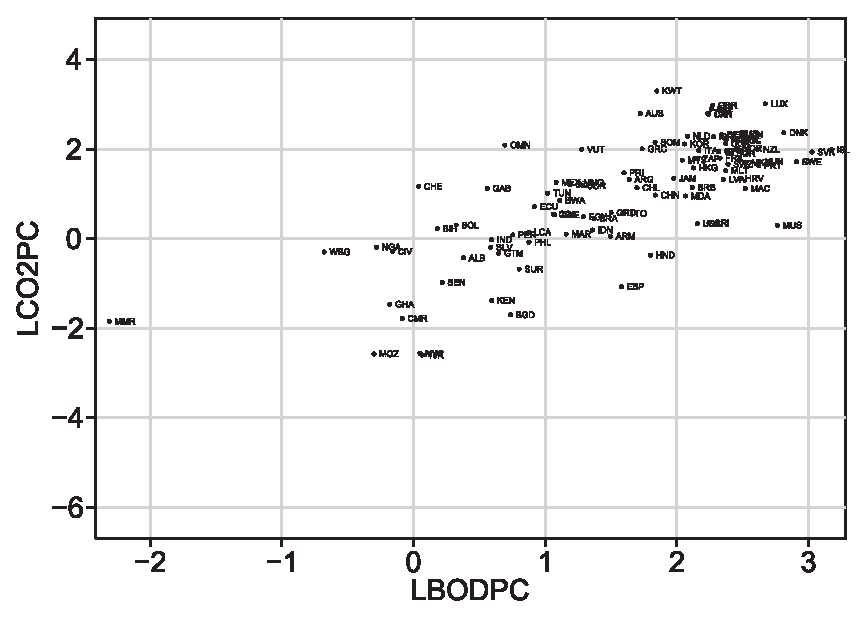
\includegraphics{flrf2.eps}
\end{center}
\caption{Fluctuations in Cohort Size $N_{t}$ over Generations.}%
\label{fig:kgrid}%
\end{figure*}

\subsection{Economic environment}

%\begin{figure}[t]
%\begin{center}
%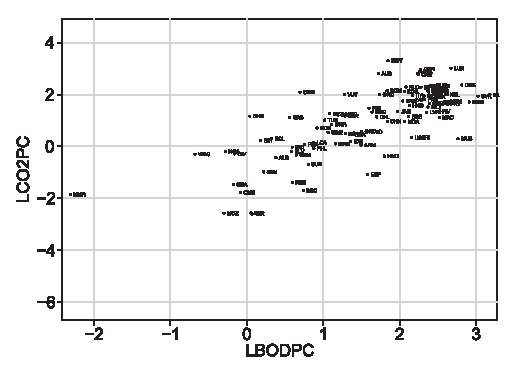
\includegraphics[width=20pc]{flrf1.eps}
%\end{center}
%\caption{Dynamics of Labor Force $L_{t}$\figsource{A group of young agents in period $t$ (i.e.,
%those who are born in period $t-1$) is
%called generation $t$, and its cohort size is denoted by $N_{t}$.}}%
%\label{fig:labordynamics}%
%\end{figure}

Agents undertake no economic activity in their childhood, supply one unit of
labor inelastically in their youth and middle age, respectively, and retire
when old. The total labor force in period $t$ is thus expressed as:
\begin{equation}
L_{t}=N_{t}+N_{t-1}, \label{eq:labor}%
\end{equation}
which is depicted in Fig.~1 for various levels of $\lambda$. This figure shows that the delayed
childbearing decreases the labor force permanently even when the lifetime fertility rate is held
constant, and the level of $L_{t}$ is lower when a larger fraction of agents decide to delay
childbearing (i.e., when $\lambda$ is higher). {Using $N_{t}=\frac {1}{1+\lambda}\left( 1+\left(
-1\right)  ^{t}\lambda^{t+1}\right)  $, the total labor force is expressed as $L_{t}=
\frac{1}{1+\lambda}\left(  2+\left( -1\right)  ^{t-1}\lambda^{t}\left(  1-\lambda\right)  \right)
$ for $t\geq1$. In period 0, it is given by $2-\lambda$. It can be shown analytically that $L_{t}$
is a decreasing function with respect\vs{1} to $\lambda$ when $0\leq \lambda\leq1$. Similarly, the
total population,\vs{1} ${\textstyle\sum \nolimits_{j=-1}^{2}} N_{t-j}$, also decreases as
$\lambda$ increases.} Observe also that the labor force $L_{t}$ has much smaller oscillations than
the cohort size $N_{t}$ (in fact, there is no oscillation when $\lambda=1$). We will show that the
fluctuations in the age composition of the labor force, rather than in the size of the labor force
itself, drive the economic dynamics in this model.



There is a single final good in each period that can be used for either consumption or investment.
Consumption takes place when agents are middle-aged and old. {For simplicity, we do not explicitly
consider consumption in childhood and youth as the main results are not qualitatively affected. We
also ignore the utility from and the costs of having children. See, for example, Tamura (2006) for
the fertility decision through utility maximization.} The utility of a generation-$t$ agent is
given by:
\begin{equation}
U_{t}= \log c_{m,t+1}+\beta\log c_{o,t+2}, \label{eq:U}%
\end{equation}
where $c_{m,t+1}$ and $c_{o,t+2}$ represent generation-$t$ consumption in
their middle age (period $t+1$) and old age (period $t+2$), respectively.

Let $w_{t}$ and $r_{t}$ denote the wage rate and the gross interest rate
(i.e., including the principal) in period $t$. Then, the budget constraint of
a generation-$t$ agent is:%
\begin{align}
a_{y,t}  &  =w_{t},\label{eq:budget1}\\
c_{m,t+1}+a_{m,t+1}  &  =w_{t+1}+r_{t+1}a_{y,t},\label{eq:budget2}\\
c_{o,t+2}  &  =r_{t+2}a_{m,t+1}, \label{eq:budget3}%
\end{align}
where $a_{y,t}$ and $a_{m,t+1}$ denote the amounts of assets held by a
generation-$t$ agent when she is young and middle-aged, respectively.
Maximizing (\ref{eq:U}) subject to (\ref{eq:budget1})-(\ref{eq:budget3})
yields:
\begin{align}
c_{m,t+1}  &  =(1-z) \left(  r_{t+1}w_{t}+w_{t+1}\right)  ,\label{eq:c2}\\
a_{m,t+1}  &  =z \left(  r_{t+1}w_{t}+w_{t+1}\right)  , \label{eq:a2}%
\end{align}
where $z\equiv{\beta}/({1+\beta})$ denotes the propensity to save by the
middle-aged, which is a key parameter in the following analysis.

Observe that in period $t$, aggregate savings consist of the asset holdings of
young agents, $a_{y,t}N_{t}$, and the assets held by the middle-aged,
$a_{m,t}N_{t-1}$. These aggregate savings, denoted by $S_{t}$, become the
capital stock in the next period. From (\ref{eq:budget1}) and (\ref{eq:a2}),
this means that the capital stock in period $t+1$, denoted by $K_{t+1}$, is
determined as:
\begin{equation}
K_{t+1} =S_{t}= a_{y,t}N_{t}+a_{m,t}N_{t-1} =w_{t} N_{t} + z (r_{t}
w_{t-1}+w_{t})N_{t-1}. \label{eq:asset}%
\end{equation}


Goods are produced competitively by a representative firm using labor and the
capital stock. The aggregate amount of production is given by a standard
Cobb--Douglas production function $Y_{t} = AK_{t}^{\alpha}L_{t}^{1-\alpha}$,
where parameter $A>0$ is total factor productivity, whereas parameter
$\alpha\in(0,1)$ represents the share of capital. The production function can
be expressed in terms of per-worker values as $y_{t}= Ak_{t}^{\alpha}$, where
$y_{t}\equiv Y_{t}/L_{t}$ is output per worker and $k_{t}\equiv K_{t}/L_{t}$
is the capital--labor ratio. Denoting the capital depreciation rate by
$\delta\in\left[  0,1\right]  $, the profit-maximizing condition for the firm
implies that the factor prices in equilibrium are:%
\begin{align}
r_{t}  &  =A\alpha k_{t}^{\alpha-1}+1-\delta\equiv r\left(  k_{t}\right)
,\label{eq:r}\\
w_{t}  &  =A\left(  1-\alpha\right)  k_{t}^{\alpha} \equiv w\left(
k_{t}\right)  . \label{eq:w}%
\end{align}


Substituting these factor prices into (\ref{eq:asset}) gives the evolution of
per-worker capital over generations:
\begin{equation}
k_{t+1}=A\left(  1-\alpha\right)  \frac{N_{t}k_{t}^{\alpha}+zN_{t-1}  }{N_{t+1}+N_{t}}, \label{eq:Dyn_k^2_Grand}%
\end{equation}
where we used the fact that $k_{t+1}=K_{t+1}/L_{t+1}=K_{t+1}/(N_{t+1}+N_{t})$.
Recalling that the timing of childbirth $\lambda_{t}$ for all $t$ is given by
(\ref{eq:lambda}), equation (\ref{eq:PopDyn}) and initial condition
$N_{-1}=N_{0}=1$ determine the demographic dynamics $N_{t}$ for all $t$. Then,
given the path of $N_{t}$ and the initial two values of capital, $k_{0}$ and
$k_{-1}$, (\ref{eq:Dyn_k^2_Grand}) determines the dynamic path of the
capital--labor ratio $k_{t}$ for all $t$.

\section{Dynamic Effects of Delayed Childbearing\label{sec:Dyn}}

In the following, we investigate the dynamic effects of delayed childbearing
on capital accumulation and welfare. Throughout this section, we focus on the
polar case of $\lambda=1$, where all agents beginning from generation 0 bear
children in middle age. Although this case is not very plausible, it allows us
to analytically explain the effect of delaying childbearing in a simple way.
We also assume full capital deprecation ($\delta=1$) in this section. The
general case with $\lambda,\ \delta\in\left(  0,1\right)  $ will be
numerically investigated in the next section.

\subsection{ Equilibrium path when all agents delay childbearing
\label{subsec:Dyn_Property}}

\begin{table*}[!t]
\tableparts{\caption{Evolution of Demographic Structure When $\lambda=1$. Numbers in Italic
Indicate the Cohorts in the Labor Force\label{table:lambda_1}}}
{\tabcolsep=0pt\begin{tabular*}{\textwidth}{@{\extracolsep{\fill}}lccccc@{}}\toprule
& Period  & Period &  Period &  Even periods  &  Odd periods\\
& --1 &  0  &  1  & $\boldsymbol{t=2,4,\dots}$ & $\boldsymbol{t=3,5,\dots}$\\\colrule
 Old & 1 & 1 & 1 & 1 & 0\\[.1pt]
 Middle-Aged (worker) & \textit{1} & \textit{1} & \textit{1} &
\textit{0} & \textit{1}\\
\textit{Young (worker)} & \textit{1} & \textit{1} & \textit{0} & \textit{1} &
\textit{0}\\
Child & 1 & 0 & 1 & 0 & 1\\\botrule
\end{tabular*}}
{\tablenote{Therefore, they earn the entire output $Y_{t}$. The middle-aged are the sole savers in
odd periods, and they save fraction $z$ of their income. Throughout this section, we focus on the
polar case of $\lambda=1$, where all agents beginning from generation 0 bear children in middle
age. }}
\end{table*}

When $\lambda=1$, the demographic dynamics (\ref{eq:PopDyn}) simplify to $N_{t+1}=N_{t-1}$ for all
$t \geq1$. Substituting $N_{0}=1$ and $N_{1}=0$ from (\ref{eq:N1}) into this equation, it turns
out that $N_{t}=1$ for all even $t$ and $N_{t}=0$ for all odd $t$. Table \ref{table:lambda_1}
describes the implied demographic structure at each point in time. Note that the whole labor force
consists only of young workers in even periods, and only of middle-aged workers in odd periods.
{Of course, this is an extreme possibility: young and middle-aged workers would coexist if
$\lambda\in\left(  0,1\right) $. However, the important point is that the composition of young and
middle-aged workers in the labor force fluctuates, which is still true for $\lambda\in(0,1)$.
Observe from the demographic dynamics illustrated by Fig.~2 that the young workers are the
majority (i.e., $N_{t}>N_{t-1}$) in the even periods, whereas the middle-aged workers are the
majority (i.e., $N_{t}<N_{t-1}$) in the odd periods.}

With the path of $N_{t}$, we can derive the equilibrium path of the capital--labor ratio $k_{t}$,
given the initial $k_{0}$ and $k_{-1}$ values. Substituting $N_{0}=N_{-1}=1$ and $N_{1}=0$ into
(\ref{eq:Dyn_k^2_Grand}) for $t=0$, we obtain the capital--labor ratio in period 1: {Recall also
that we have assumed $\delta=1$ for this section.}
\begin{equation}
k_{1}=A(1-\alpha)\left[  (1+z)k_{0}^{\alpha}+zA\alpha k_{0}^{\alpha-1}%
k_{-1}^{\alpha}\right]  . \label{eq:Dyn_k^2_Period1}%
\end{equation}
%For $k_{2}$ and onwards, substituting $\left\{  N_{0},N_{1},N_{2},N_{3}%
%,\cdots\right\}  =\left\{  1,0,1,0,\cdots\right\}  $ into
%(\ref{eq:Dyn_k^2_Grand}) gives:
%\begin{equation}
%\text{for $t \geq1,$}\quad k_{t+1}=\left\{
%\begin{array}
%[c]{ll}%
%A\left(  1-\alpha\right)  k_{t}^{\alpha} & \text{if $t$ is even},\\
%A\left(  1-\alpha\right)  z\left\{  k_{t}^{\alpha}+A\alpha k_{t-1}^{\alpha
%}k_{t}^{\alpha-1}\right\}  & \text{if $t$ is odd}.
%\end{array}
%\right.  \label{eq:Dyn_k^2_Lambda=1}%
%\end{equation}


This pattern of dynamics can be intuitively interpreted in terms of the
aggregate saving rate (adjusted for labor force growth), defined by:
\begin{equation}
v_{t}\equiv\frac{S_{t}}{Y_{t}}\left/  \frac{L_{t+1}}{L_{t}}\right.  =
\frac{K_{t+1}/L_{t+1}}{Y_{t}/L_{t}} =\frac{k_{t+1}}{A k_{t}^{\alpha}}.
\label{eq:v}%
\end{equation}
As labor force $L_{t}$ is constant at 1 for all $t\geq1$ (see Fig.~1), $v_{t}$ simply represents
the aggregate saving rate for $t\geq1$.

Using this definition, the first line of equation (\ref{eq:Dyn_k^2_Lambda=1})
can be restated as $v_{t}=1-\alpha$. In even periods, young agents are the
sole workers, and thus they earn the labor share of output, $(1-\alpha) Y_{t}%
$. At the same time, they are also the sole savers in even periods, and
because they save their income entirely, aggregate savings coincide with their
income, $(1-\alpha)Y_{t}$. Therefore, in even periods, the aggregate saving
rate $v_{t}$ is determined by the labor share of the production, $1-\alpha$.

\begin{flthem}
The middle-aged are the sole savers in odd periods, and they save fraction $z$ of their income.
Therefore, the aggregate saving rate $v_{t}$ coincides with their saving propensity, $z$. {When
$\lambda\in(0,1)$, labor force $L_{t}$ does fluctuate in transition dynamics. However, comparing
Figs~1 and 2 shows that the fluctuations in labor force $L_{t}$ are much smaller than in the
demographic dynamics of $N_{t}$.}
\end{flthem}


For odd periods, the second line of equation (\ref{eq:Dyn_k^2_Lambda=1}) can
be restated as $v_{t}=\left(  1-\alpha\right)  z \left(  1+{\alpha}/{v_{t-1}%
}\right)  $. Note that $v_{t-1}$ in this equation refers to the aggregate saving rate in even
periods, which is $1-\alpha$ as shown above. By substituting $v_{t-1}=1-\alpha$ into the above
equation, it simplifies to $v_{t}=z$. In odd periods ($t\geq3$), the middle-aged are the only
workers. In addition, the capital used in odd periods is owned solely by the middle-aged, because
they are the only savers in the previous period (when they were young in even periods). Therefore,
they earn the entire output $Y_{t}$.

\begin{flLem}
The middle-aged are the sole savers in odd periods, and they save fraction $z$ of their income.
Therefore, the aggregate saving rate $v_{t}$ coincides with their saving propensity, $z$. {When
$\lambda\in(0,1)$, labor force $L_{t}$ does fluctuate in transition dynamics. However, comparing
Figs~1 and 2 shows that the fluctuations in labor force $L_{t}$ are much smaller than in the
demographic dynamics of $N_{t}$.}
\end{flLem}

To summarize, the aggregate saving rate $v_{t}$ exhibits a two-period cycle after period 2: {There
is no cycle in the knife-edge case of $1-\alpha=z$. For completeness, $v_{0}$ is obtained by
$v_{0}= k_{1}/\left( Ak_{0}^{\alpha}\right)  $, where $k_{0}$ is a part of the initial condition
and $k_{1}$ is given by (1). The level of $v_{1}$ is
then obtained by $v_{1}=\left(  1-\alpha\right)  z \left(  1+{\alpha}/{v_{0}%
}\right)  .$ \label{foot:v}}
\begin{equation}
\text{for $t\geq2$,}\quad v_{t}=\left\{
\begin{array}
[c]{cl}%
1-\alpha & \text{if $t$ is even},\\
z & \text{if $t$ is odd}.
\end{array}
\right.  \label{eq:v_t}%
\end{equation}
Note that either the saving rate in even periods $1-\alpha$, or that in odd
periods $z$, could be larger. On one hand, young workers have a high saving
propensity (unity), but they save only out of labor income ($w_{t}$). On the
other hand, middle-aged workers earn both labor and capital income
($w_{t}+r_{t}w_{t-1}$), but their saving propensity is lower ($z<1$%
). {From the Family Income and Expenditure Survey for wage-earning households with two or more
persons in Japan, we confirmed that the average saving rate (1$-$ the average propensity to
consume) tends to fall with the age of the household head, from 32.0\% (thirties) to 28.8\%
(forties) to 25.4\% (fifties) and then to 11.3\% (sixties) using 2000--2010 data. While some other
reports find flat or rising age-saving profiles (even after the retirement age), Jappelli and
Modigliani (2005) pointed out that these are because contributions to pension funds (including
employers' contribution) are not regarded as savings, and also because pension incomes are treated
as income although they should be regarded as dissavings. They estimated the effects of social
security on the age-saving profile in Italy, which showed that actual savings are highest when the
household head is in his/her late thirties and then falls to zero around age 60.}

Using the values of $v_{t}$ in (\ref{eq:v_t}), we can derive the sequence of
$k_{t}$. Note that (\ref{eq:v}) implies a simple relationship between the
aggregate saving rate $v_{t}$ and the evolution of the capital--labor ratio
$k_{t}$:
\begin{equation}
k_{t+1}=v_{t}Ak_{t}^{\alpha}. \label{eq:Dyn_v_k}%
\end{equation}
Taking the logs of (\ref{eq:Dyn_v_k}) and applying this recursively, we
obtain:
\begin{equation}
\log k_{t}=\left(  \sum_{j=0}^{t-3}\alpha^{j}\right)  \log A+\left(
\sum_{j=0}^{t-3}\alpha^{j}\log v_{t-1-j}\right)  +\alpha^{t-2}\log k_{2}, \label{eq:ksequence}%
\end{equation}
where $k_{2}=A(1-\alpha)z\left\{  k_{1}^{\alpha}+A\alpha k_{0}^{\alpha}%
k_{1}^{\alpha-1}\right\}  $ from (\ref{eq:Dyn_k^2_Lambda=1}), $k_{1}$ is given by (1), and $k_{0}$
(and $k_{-1}$) is given as the initial value. This equilibrium path has the following property.

\begin{flLem}
In the equilibrium with $\lambda=1$, $\left\{ k_{t}\right\} _{t=0}^{\infty}$ converges to a
two-period limit cycle regardless of the initial values. Define $k_{even}^{\ast}\equiv\lim
_{s\rightarrow+\infty}k_{2s}$ and $k_{odd}^{\ast}\equiv\lim_{s\rightarrow +\infty}k_{2s+1}$, where
$s$ is an integer. Depending on $z\equiv \beta/(1+\beta)$, the relative magnitude of
$k_{even}^{\ast}$ and
$k_{odd}^{\ast}$ is:\newline\textrm{(Case I)} if $z<1-\alpha$, $k_{even}%
^{\ast}<k_{odd}^{\ast}$ holds.\newline\textrm{(Case II)} if $z>1-\alpha$,
$k_{even}^{\ast}>k_{odd}^{\ast}$ holds. {\label{fn:caseII}}
\end{flLem}

\begin{proof}
As $t\rightarrow\infty$, the first term of (\ref{eq:ksequence}) converges to
$(1-\alpha)^{-1}\log A$, whereas the third term vanishes because $\alpha
\in(0,1)$. When $t$ is even (i.e., when $t=2s$ for some integer $s$), from
(\ref{eq:v_t}), the second term is expanded as $\log z+\alpha\log
(1-\alpha)+\alpha^{2}\log z+\alpha^{3}\log(1-\alpha)+\cdots,$ which converges
to $(1-\alpha)^{-1}\log V_{even}(z)$, where:
\begin{equation}
V_{even}(z)\equiv\left[  \left(  1-\alpha\right)  ^{\alpha}z\right]
^{\frac{1}{1+\alpha}} \label{eq:V_even}%
\end{equation}
is a geometric weighted average of the aggregate saving rate $v_{t}%
$. {Observe that $V_{even}(z)$ in (\ref{eq:V_even}) puts a higher weight on $z$ than on
$(1-\alpha)$ because in even periods the most recent aggregate saving rate is $v_{2s-1}=z$.
Similarly, $V_{odd}(z)$ in (\ref{eq:V_odd}) puts a higher weight on $(1-\alpha)$.} Similarly, when
$t$ is odd (i.e., when $t=2s+1$), the second term is expanded as $\log(1-\alpha )+\alpha\log
z+\alpha^{2}\log(1-\alpha)+\alpha^{3}\log z+\cdots,$ which converges to $(1-\alpha)^{-1}\log
V_{odd}(z)$, where:
\begin{equation}
V_{odd}(z)\equiv\left[  \left(  1-\alpha\right)  z^{\alpha}\right]  ^{\frac
{1}{1+\alpha}}. \label{eq:V_odd}%
\end{equation}
From these, we conclude that the values of $k_{t}$ in even and odd periods,
respectively, converge to:
\begin{align}
&  \lim_{s\rightarrow\infty}\log k_{2s}=\log k_{even}^{\ast}=\frac{1}%
{1-\alpha}\left[  \log V_{even}(z)+\log A\right]  ,\label{eq:Logk*_Even}\\
&  \lim_{s\rightarrow\infty}\log k_{2s+1}=\log k_{odd}^{\ast}=\frac
{1}{1-\alpha}\left[  \log V_{odd}(z)+\log A\right]  . \label{eq:Logk*_Odd}%
\end{align}
Note that $V_{even}(z)<V_{odd}(z)$ holds if $z<1-\alpha$ (Case I), whereas the
opposite holds if $z>1-\alpha$ (Case II). Therefore, $k_{even}^{\ast}%
<k_{odd}^{\ast}$ holds if and only if $z<1-\alpha$.
\end{proof}

%\begin{figure}[ptb]
%\begin{center}%
%\begin{tabular}
%[c]{ll}%
%(i) Case I: $z<1-\alpha$ & (ii) Case II: $z>1-\alpha$\\
%%\includegraphics[width=.5 \textwidth]{fig3i_limit_caseI.eps}
%&
%%\includegraphics[width=.5 \textwidth]{fig3ii_limit_caseII.eps}
%\end{tabular}
%\end{center}
%\caption{Limit Cycles in $k_{t}$ with Alternating Aggregate Saving Rate
%$v_{t}$.}%
%\label{fig:lambda=1}%
%\end{figure}

Proposition~1 states that if all agents from period 0 delay childbearing, the capital--labor ratio
$k_{t}$ eventually converges to a two-period limit cycle. This fluctuation is driven not by the
size of the labor force (which is constant), but by the age distribution within it, through the
fluctuations in the aggregate saving rate $v_{t}$. Figure~1 illustrates the limit cycles for the
two cases, where the two loci are drawn by substituting $1-\alpha$ (even periods) and $z$ (odd
periods) for $v_{t}$ in the capital accumulation equation (\ref{eq:Dyn_v_k}). Panel (i) shows that
in Case I ($z<1-\alpha$), the aggregate saving rate is higher in even periods, which results in a
higher capital stock in odd periods. Conversely, panel (ii) depicts that the higher saving rate in
odd periods results in the higher capital stock in even periods in Case II ($z>1-\alpha$).

%It is worth noting that we consider a quartet weight as an estimation of the sum of the weights of
%all splits displaying that quartet. This corresponds to the length of the middle edge of the
%corresponding quartet tree (see also Gru�newald et al. 2007). There are a number of studies that
%define a quartet weight to be the confidence in or likelihood of a quartet topology under
%variousmodels of sequence evolution (Willson 1999; Ranwez and Gascuel 2001; Huson et al. 2004;
%Sumner et al. 2008; Holland et al. 2007, 2008, 2013; Snir and Rao 2012). In the implementation of
%Quartet-Net, the following two options are provided: 1) construct a split network directly from
%the sequence alignment file using the parsimony method on informative sites to calculate triplet
%and quartet weights; and 2) construct a split network from a triplet and quartet file in a given
%format (see user�s manual), specifying the triplet and quartet weights precomputed by the user.
%
%The main purpose of the second option is to separate the two steps of the algorithm, the
%computation of triplet and quartet weights from an MSA and the computation of a split system from
%this intermediate data. We simply count site patterns to assign quartet weights. Similarly, the
%simple uncorrected P distance is commonly used for Neighbor-Net and Split Decomposition, for
%example, it is the default distance of SplitsTree v4 (Huson and Bryant 2006). Other quartet
%weights have been suggested. QNet (Gru�newald et al. 2007) comes with a procedure that utilizes
%the maximum likelihood framework of Tree Puzzle (Strimmer and von Haeseler 1997) to compute
%�expected branch lengths,� quartet weights that converge to the true value, if the sequences
%evolve along a tree under the GTR model. More recently, (Holland et al. 2013) used �squangles� to
%estimate quartet weights under the general Markov model. These modelbased ways to compute quartet
%weights might be very useful, if the true underlying split system is a tree. If not, then the
%violation of the underlying compatibility assumption of the models can be a problem. This is
%indicated by the relatively high weight of the wrong splits for QNet with �expected branch
%lengths� in our simulation.

\subsection{Effects on capital accumulation\label{subsec:Compare}}

As we have seen in Fig.~1, delayed childbearing lowers the labor force permanently. This
subsection examines how this affects capital accumulation in the economy by comparing the
capital--labor ratio in the limit cycles to the economy without delayed childbearing.

Note that without delayed childbearing (i.e., when $\lambda=0$), $N_{t}=1$
holds for all $t$ from (\ref{eq:PopDyn}) and the initial condition $N_{0}=1$.
By substituting $N_{t-1}=N_{t}=N_{t+1}=1$ and $\delta=1$ into the capital
accumulation equation (\ref{eq:Dyn_k^2_Grand}), and rewriting the resulting
equation using $v_{t}\equiv k_{t+1}/(Ak_{t}^{\alpha})$, we obtain the
evolution of the aggregate saving rate $v_{t}$ for the case of $\lambda=0$.
From it, we find that the steady state level of $v_{t}$ is a (positive)
solution to a quadratic equation $\xi\left(  v\right)  \equiv2v^{2}-\left(
1-\alpha\right)  \left(  1+z\right)  v-\alpha\left(  1-\alpha\right)  z=0,$
which we obtain as:
\begin{equation}
v^{\ast}(z)\equiv\frac{1}{4}\left\{  \left(  1-\alpha\right)  \left(
1+z\right)\right\}  .\label{eq:v*}%
\end{equation}
Solving  $k^{\ast}/(A\left(  k^{\ast}\right)  ^{\alpha})=v^{\ast}(z)$ for
$k^{\ast}$, the steady state capital--labor ratio for $\lambda=0$ is obtained
as:
\begin{equation}
\log k^{\ast}=\frac{1}{1-\alpha}\left[  \log v^{\ast}(z)+\log A\right]
.\label{eq:Logk*}%
\end{equation}


It is apparent from (\ref{eq:Logk*_Even}), (\ref{eq:Logk*_Odd}) and
(\ref{eq:Logk*}) that the relative magnitudes of the capital--labor ratios,
$k_{odd}^{\ast}$, $k_{even}^{\ast}$, and \noindent$k^{\ast}$, can be obtained
by comparing $V_{odd}(z)$, $V_{even}(z)$, and $v^{\ast}(z)$. To focus on the
relevant situation, we assume that the share of capital is not too high:
$\alpha<\left(  \sqrt{5}-1\right)  /2 \approx0.618$. With this assumption, we
can show the following property.

\begin{flLem}
\label{lm:Comparison}\textrm{(i)} At $z=1-\alpha$, $V_{odd}(z)=V_{even}(z)=v^{\ast}(z)=1-\alpha$
holds.\newline\textrm{(ii)} There exist $\widehat{z}\in\left(  0,1-\alpha\right)  $ such that
$V_{odd}(\widehat z)=v^{\ast}(\widehat z)$ holds. $V_{odd}(z)>v^{\ast}(z)$ holds if and only if $z
\in(\widehat{z}, 1-\alpha)$.
\newline\textrm{(iii)} $V_{even}(z)>v^{\ast}(z)$ holds if and only if $z>1-\alpha$.
\end{flLem}

\begin{proof}
Property (i) is immediately confirmed by comparing (\ref{eq:V_even}),
(\ref{eq:V_odd}), and (\ref{eq:v*}) at $z=1-\alpha$. The proofs of (ii) and
(iii) are given in Appendix 1.
\end{proof}

%\begin{table}[t]
%\tableparts{\caption{Derivation of Proposition
%\ref{prop:Comparison} from Proposition \ref{prop:lambda=1} and
%Lemma \ref{lm:Comparison}\label{table:Lemma1}}}
%{\begin{tabular*}{\textwidth}{@{\extracolsep{\fill}}lccc@{}}\toprule%
%{Range of ${z}$} & ${z<\widehat z}$ & ${\widehat z<z<1-\alpha}$ & ${1-\alpha<z}$\\\colrule
%Proposition \ref{prop:lambda=1} & \multicolumn{2}{c|}{$k^{*}_{even}%
%<k^{*}_{odd}$} & $k^{*}_{odd}<k^{*}_{even}$\\
%Lemma \ref{lm:Comparison}(ii) & $k^{*}_{odd}<k^{*}$ & $k^{*}<k^{*}_{odd}$ &
%$k^{*}_{odd}<k^{*}$\\
%Lemma \ref{lm:Comparison}(iii) & \multicolumn{2}{c|}{$k^{*}_{even}<k^{*}$} &
%$k^{*}<k^{*}_{even}$\\
%Proposition \ref{prop:Comparison} & $k^{*}_{even}<k^{*}_{odd}<k^{*}$ &
%$k^{*}_{even}<k^{*}<k^{*}_{odd}$ & $k^{*}_{odd}<k^{*}<k^{*}_{even}$\\
%& (Case Ia) & (Case Ib) & (Case II)\\\botrule
%\end{tabular*}}
%%\includegraphics[width=\textwidth]{table2_derivation.eps}
%{}
%%
%\end{table}

As summarized in Table~1, Proposition~1 and Lemma~1 imply three possibilities regarding the
relative magnitudes of $k_{odd}^{\ast}$, $k_{even}^{\ast}$, and \noindent$k^{\ast}$: {It can also
be shown that if $z=1-\alpha$ (i.e., when capital does not fluctuate),
$k_{even}^{\ast}=k_{odd}^{\ast}=k^{\ast}$
holds. In addition, if $z=\widehat z$, $k_{even}^{\ast}<k_{odd}^{\ast}%
=k^{\ast}$ holds. We ignore these border cases because they do not occur
except for a (measure 0) coincidence.}

%\begin{Prop}[Comparison of capital--labor ratios
%between the limit cycle at $\lambda=1$ and the steady state at $\lambda=0$:]
%\label{prop:Comparison} \textrm{(Case Ia)} If $z< (0,\widehat{z})$, $k_{even}^{\ast}%
%<k^{*}_{odd}<k^{\ast}$ holds.\newline\textrm{(Case Ib)} If $z<(\widehat{z},
%1-\alpha)$, $k_{even}^{\ast}<k^{\ast}<k^{*}_{odd}$ holds.\newline\textrm{(Case
%II)} If $z>1-\alpha$, $k_{odd}^{\ast}<$\textit{\noindent}$k^{\ast}%
%<k_{even}^{\ast}$ holds.
%\end{Prop}

Observe that the lower end of the limit cycle ($\min\{k_{odd}^{\ast}%
,k_{even}^{\ast}\}$) is always smaller than the steady state level $k^{\ast}$ in the economy
without delayed childbearing (which we call the benchmark economy). In addition, if $z$ is
sufficiently small ($z<\widehat z$), the upper end of the limit cycle can also be smaller than
$k^{\ast}$. This means that the long-term levels of the capital--labor ratio $k_{t}$ in the
delayed childbearing economy are always smaller than the steady state capital--labor ratio $k^{*}$
in the benchmark economy. This might seem paradoxical, given that in the delayed childbearing
economy, the labor force remains low compared with the benchmark economy (compare $\lambda=1$ to
$\lambda=0$ in Fig.~1). This paradoxical result can be explained by the alternating age
composition in the labor force. Recall from (\ref{eq:v_t}) that the aggregate saving rate
alternates between $1-\alpha$ and $z$. In Case Ia, the saving propensity of the middle-aged
agents, $z\equiv\beta/(1+\beta)$, is small. Thus, in odd periods, when the labor force is entirely
composed of middle-aged agents, the aggregate saving rate $v_{t}=z$ is low. This makes capital per
worker in the next period ($k^{*}_{even}$) considerably smaller than in the benchmark ($k^{*}$),
and therefore also the wage rate. As a result, workers in even periods, who are composed of young
agents, receive substantially lower incomes than in the benchmark economy. Thus, even though the
aggregate saving rate in even periods $v_{t}=1-\alpha$ is higher than that in the benchmark
economy ($v^{*}(z)$), the amount of aggregate savings can be
lower, which explains the possibility of $k^{*}_{even}<k^{*}_{odd}<k^{*}%
$. {One may then wonder why $k^{\ast}<k_{odd}^{\ast}<k_{even}^{\ast}$ never occurs in Case II. As
we assumed $\alpha$ to be lower than $\left( \sqrt{5}-1\right)  /2$, the wage equation
$w_{t}=A(1-\alpha)k_{t}^{\alpha}$ has a certain degree of concavity with respect to $k_{t}$. This
concavity implies that, while a negative deviation $k^{*}_{even}$ from $k^{\ast}$ in Case I
results in a substantial drop in the wage income, a positive deviation of $k^{*}_{even}$ from
$k^{\ast}$ in Case II results in a relatively small wage increase. Therefore, $k_{odd}^{\ast}$
does not exceed $k^{\ast}$ in Case II. \label{foot:K_Flu_Effect}}

\subsection{Welfare effects\label{sec:Welfare}}

We now examine how the cycles in the capital--labor ratio in the delayed
childbearing economy affect the welfare of agents. Note that, by substituting
(\ref{eq:budget3}), (\ref{eq:c2}), and (\ref{eq:a2}) into (\ref{eq:U}), the
utility of generation-$t$ agents (those who are born in period $t-1$) is
written as:
\begin{equation}
U_{t}=\beta\log z+\log(1-z)+(1+\beta)\log\left(  r_{t+1}w_{t}+w_{t+1}\right). \label{eq:welfare}%
\end{equation}
Let us call those agents born in odd periods and thus young in even periods
the `even-period generations.' In the delayed childbearing economy
($\lambda=1$), the whole population is composed only of the even-period
generations ($N_{t}=0$ for all odd $t$). Therefore, the long-term welfare of
agents in the limit cycle can be measured by $U_{even}^{\ast}\equiv
\lim_{s\rightarrow+\infty}U_{2s}$. Using the limit-cycle values of the
capital--labor ratio, we can write long-term welfare with $\lambda=1$ as:
\begin{equation}
U_{even}^{\ast}=\left(  1+\beta\right)  \log[A\alpha\left(  k_{odd}^{\ast
}\right)  ^{\alpha-1}\left(  k_{even}^{\ast}\right)  ^{\alpha}+\left(
k_{odd}^{\ast}\right)  ^{\alpha}], \label{eq:U_even}%
\end{equation}
where $C$ is a constant term defined as $C\equiv\beta\log\beta-(1+\beta
)\log(1+\beta)+\beta\log A\alpha+(1+\beta)\log A\left(  1-\alpha\right)  $.
Similarly, long-term welfare in the benchmark economy ($\lambda=0$) can be
written as:
\begin{equation}
U^{\ast}=\left(  1+\beta\right)  \log[A\alpha\left(  k^{\ast}\right)
^{2\alpha-1}+\left(  k^{\ast}\right)  ^{\alpha}]-\beta\left(  1-\alpha\right)
\log k^{\ast}+C. \label{eq:U_benchmark}%
\end{equation}


Comparing (\ref{eq:U_even}) with (\ref{eq:U_benchmark}), we have the following property.

%\begin{Lm}
%\label{lm:Omega} \textrm{\textbf{(Difference between $U^{*}_{even}$ and
%$U^{*}$):}}\newline\textrm{(i)} $U^{*}_{even}$ is lower than $U^{*}$ if and
%only if $\Omega(z)<0$, where function $\Omega(z)$ is defined by:
%\begin{equation}
%\Omega\left(  z\right)  \equiv-\log\left(  1-\alpha\right)  \left[
%\frac{\alpha}{v^{\ast}\left(  z\right)  }+1\right]  -\frac{\alpha}{1-\alpha
%}\log\frac{v^{\ast}\left(  z\right)  }{V_{odd}\left(  z\right)  }+z\log
%\frac{v^{\ast}\left(  z\right)  }{V_{even}\left(  z\right)  }.
%\label{eq:Omega}%
%\end{equation}
%\textrm{(ii)} $\lim_{z\rightarrow0}\Omega\left(  z\right)  =-\infty$ and
%$\Omega(1-\alpha)=0$ hold.
%\end{Lm}
%
%\begin{Proof}
%Given in Appendix 2.
%\end{Proof}

As function $\Omega(z)$ is continuous, Lemma~2 implies that when $z$ is sufficiently close to $0$,
$\Omega(z)$ must be negative, and hence $U^{*}_{even}< U^{*}$ holds. The next proposition states
this result.

%\begin{Prop}
%\label{prop:welfare} \textrm{\textbf{(Welfare comparison between $\lambda=1$
%and $\lambda=0$):}}\newline There exists a value $\widetilde z \in
%(0,1-\alpha]$ such that $U^{*}_{even}<U^{*}$ holds whenever $z<\widetilde z$.
%\end{Prop}

As long as the saving propensity of the middle-aged, $z\equiv\beta/(1+\beta)$,
is sufficiently small, or equivalently when the agents discount the future
significantly (i.e., $\beta$ is small), the delayed childbearing ($\lambda=1$)
causes the long-run welfare of agents to fall compared with the case where
delayed childbearing does not occur ($\lambda=0$). This again seems
paradoxical, because when the population falls from the initial level, it is
usually anticipated that each agent enjoys a higher per-worker capital and
hence higher consumption. This does not hold true in this case, similar to the
discussion in the previous subsection, because of the fluctuations in the age
composition of workers.

\section{Numerical Analysis\label{sec:Numerical}}

This section considers a general case where only a fraction of agents delay childbearing. When
$\lambda\in(0,1)$, the fluctuations in $N_{t}$ gradually settle to a long-term value (see Fig.~2).
Nonetheless, the fluctuations in $N_{t}$ continue for an extended number of generations,
especially when $\lambda$ is relatively large. {For example, if 80\% of agents delay childbearing
($\lambda=0.8$), it can be seen that substantial fluctuations in $N_{t}$ remain even after 10
generations (around 200 years).} This section examines their effects on capital accumulation and
welfare in the transitional dynamics. We also relax the assumption of complete capital
depreciation.

\subsection{Equilibrium dynamics under \label{subsec:numerical_k}}

For a given value of $\lambda$, the path of $N_{t}$ is readily calculated as depicted in Fig.~2
using (\ref{eq:PopDyn}) and (\ref{eq:lambda}) along with initial condition $N_{0}=1$. As $N_{t}=1$
for all $t\leq0$, we reasonably assume that the economy has reached the steady state under
$N_{t}=1$ by period $-1$, and also remains at the same steady state at period 0. {Note that, even
though $\lambda_{t}$ jumps up from 0 to $\lambda>0$ in period 0, the labor force is not
immediately affected, nor is the capital--labor ratio, because the fertility in period 0
determines the amount of labor supplied in period 1 and beyond.} We previously calculated this
steady state in Subsection \ref{subsec:Compare} as the benchmark case, where the steady state
level of the capital--labor ratio $k^{\ast}$ is given by (\ref{eq:Logk*}). Thus, we use
$k_{-1}=k_{0}=k^{\ast}$ as the initial condition to calculate the path of $k_{t}$ using
(\ref{eq:Dyn_k^2_Grand}).

We specify the parameters as follows. As an agent lives for four periods, one period in the model
can be considered as approximately 20 years. If agents discount future consumption by 1\% per
quarter, as is often assumed in the literature, the discount factor $\beta$ will be $(1+0.01)^{-4
\times20} \approx0.45$. Therefore, we take $\beta=0.45$ as the reference value, and also examine
the low-beta ($\beta=0.1$) and the high-beta ($\beta=0.9$) cases. For the depreciation parameter
$\delta$, Nadiri and Prucha (1996) estimated a yearly depreciation rate for the physical capital
stock of 5.9\%, and 1.2\% for the R\&D capital stock. The capital stock $K_{t}$ in our model
includes both physical and R\&D capital stocks, but these estimates suggest that a good fraction
of the aggregate capital stock that remains after 20 years would be R\&D capital. Therefore we use
a yearly depreciation rate of 2\% as a reference (which means $\delta=0.33$ for a period of 20
years), and also examine the case of a higher depreciation rate of 5\% per year ($\delta =0.64$).
The share of capital $\alpha$ is set to 0.4. {As we do not distinguish between physical and human
capital, the share of $K_{t}$, $\alpha $, should be higher than the conventionally measured share
of physical capital. Thus, we choose $\alpha=0.4$, although the value of $\alpha$ does not
substantially change the pattern of the dynamics. The scaling parameter $A$ is set to 1.5. Under
these parameter values, we confirmed that dynamic efficiency $r_{t}>1$ is always satisfied at the
steady state.}

%\begin{figure}[t]
%\begin{center}%
%\begin{tabular}
%[c]{ll}%
%(i) $\beta=0.1$, $\delta=0.33$ (low discount factor) & (ii) $\beta=0.45$,
%$\delta=0.33$ (reference)\\
%%\includegraphics[width=.5 \textwidth]{fig4i_low_beta.eps}
%&
%%\includegraphics[width=.5 \textwidth]{fig4ii_reference.eps}
%\\
%(iii) $\beta=0.9$, $\delta=0.33$ (high discount factor) & (iv) $\beta=0.45$,
%$\delta=0.64$ (high depreciation)\\
%%\includegraphics[width=.5 \textwidth]{fig4iii_high_beta.eps}
%&
%%\includegraphics[width=.5 \textwidth]{fig4iv_high_depreciation.eps}
%\end{tabular}
%\end{center}
%\caption{Evolution of Capital--Labor Ratio $k_{t}$.}%
%\label{fig:kdynamics}%
%\end{figure}

Figure~2 shows the equilibrium paths of $k_{t}$ for $\beta=$ 0.1, 0.45, and 0.9, respectively, and
also for $\delta=0.33$ and 0.64. Each panel depicts 10 paths of $k_{t}$, where each path
corresponds to the cases of $\lambda=$ 0.1, 0.2, \dots, 0.9, and 1. In period 1, the labor force
falls from 2 to $2-\lambda$ because fraction $\lambda$ of parents in the previous period decided
to delay childbearing, and hence there are only $1-\lambda$ young workers in this period. Note
also that the aggregate capital stock is the same as in the initial steady state, because it is
determined by the aggregate savings in the previous period. {This result depends on the
logarithmic period utility function, which implies that the savings of agents do not depend on the
interest rate. If the agents are more risk averse (i.e., if the intertemporal elasticity of
substitution is because they know that the interest rate in period lower than unity), the
middle-aged agents in period 0 would somewhat increase savings, because they know that the
interest rate in period 1 will be lower because of the reduced labor supply, and would want to
supplement old-age consumption by saving more. Therefore, the magnitude of the initial
fluctuations will be larger than shown in this paper.} Therefore, the initial response of the
capital--labor ratio is always positive, and $k_{1}=\left( 2/(2-\lambda)\right)  k^{*}$ is higher
when $\lambda$ is higher.

Observe from Fig.~1 that the labor force falls further in period 2 (except for the case of
$\lambda=1$, where $L_{t}$ falls to the bottom only in one period). At the same time, however, the
aggregate capital stock is also lower than the initial steady state, because there were fewer
young workers in the previous period ($N_{1}=1-\lambda$) who contributed to aggregate savings.
Figure~2 shows that the second effect dominates, and the size of the fall in $k_{t}$ at $t=2$ is
larger when $\lambda$ is larger. In addition, when $\beta$ is small (i.e., when the saving
propensity of the middle-aged $z=\beta/(1+\beta)$ is small), the major portion of the aggregate
savings depends on the savings by the young workers. Therefore, with large $\lambda$ and small
$\beta$, the fall in aggregate savings in $t=2$ is so large that $k_{2}$ falls below (or
`overshoots') the initial capital--labor ratio $k^{\ast}$. {For example, in Fig.~3, it can be
observed that $k_{2}<k^{\ast}$ occurs when $\beta=0.1$ and $\lambda\geq0.6$.}

The pattern of dynamics after period 3 depends both on $\lambda$ and $\beta$. When only a small
fraction of parents delay childbearing, the fluctuations in cohort size $N_{t}$ disappear in a
relatively short period of time. Therefore, with small $\lambda$, $k_{t}$ settles to the steady
state value $k^{\ast}$ relatively quickly, without cycles. If $\lambda$ is relatively large,
two-period cycles in $k_{t}$ are present, which last for many generations. The pattern of the
cycles is comparable to the results we obtained in Proposition~1. Figure~2(i) shows that when
$\beta$ is small, the capital--labor ratio $k_{t}$ is smaller in even periods than in odd periods,
which corresponds to Case I (a and b) in Proposition~1. In particular, the values of $k_{t}$ in
even periods are far below the steady state value $k^{\ast}$, whereas in odd periods they are
barely above $k^{\ast}$ (except for the case of $\lambda=1$, where $k_{t}$ in odd periods is also
smaller than $k^{\ast}$, as we mentioned in Case Ia in Proposition~1). This asymmetry can be
understood in terms of the reason why both $k_{even}^{\ast}$ and $k_{odd}^{\ast}$ can be lower
than $k^{\ast}$ when $z$ is small, which we discussed in Subsection \ref{subsec:Compare}.

Figure~2(iii) shows that the pattern of the cycle is opposite when $\beta$ is large. The
capital--labor ratio is larger in even periods than in odd periods, similar to Case II in
Proposition~2. When $\beta$ is at an intermediate value ($\beta =0.45$), Fig.~3(ii) suggests that
the pattern is similar to Case I if $\lambda$ is large, whereas it is similar to Case II if
$\lambda$ is intermediate (and no cycle if $\lambda$ is small). Finally, Fig.~3(iv) illustrates
that a higher $\delta$ shifts the entire path of the capital--labor ratio $k_{t}$ downwards, but
the effect of $\delta$ on the pattern of the fluctuations is not clear from this figure.

%\begin{figure}[ptb]
%\begin{center}%
%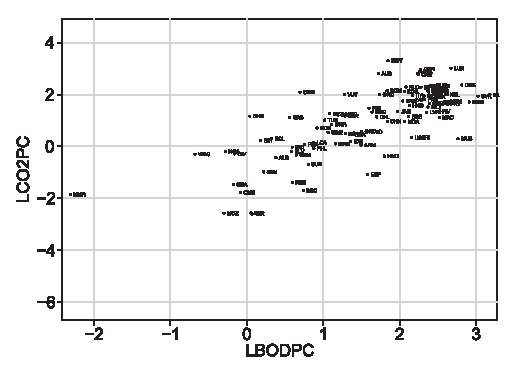
\includegraphics[width=17pc]{flrf1.eps}
%\end{center}
%\caption{Pattern of Cycles in $k_{t}$\figsource{To show the dependence of the pattern of cycles on
%parameter values more explicitly, we experimented with 40000 combinations of $\lambda$ and $\beta$
%by varying each of them from 0.005
%to 1.00 in 200 steps, and we repeated this for two values of $\delta$.}}%
%\label{fig:kgrid}%
%\end{figure}

To show the dependence of the pattern of cycles on parameter values more explicitly, we
experimented with 40000 combinations of $\lambda$ and $\beta$ by varying each of them from 0.005
to 1.00 in 200 steps, and we repeated this for two values of $\delta$. We calculated the dynamic
path of $k_{t}$ for each combination of parameters until period 10, and then classified the result
according to the pattern of movements, based on that in Proposition~3. The phase diagrams depicted
in Fig.\ \ref{fig:kgrid} summarize the result. When the combination of $\lambda$ and $\beta$
belongs to the area labeled as Case Ib, we find [$k_{t}$ in even periods] $<k^{\ast}<$ [$k_{t}$ in
odd periods] holds for all $t>3$, whereas we find [$k_{t}$ in even periods] $<$ [$k_{t}$ in odd
periods] $<k^{\ast}$ in the small area labeled as Case Ia. {As explained in the text, we classify
the pattern of the dynamics according to the level of $k_{t}$ relative to the steady state value
$k^{\ast}$. An alternative method of classification is to focus on the first difference of the
capital--labor ratio, $k_{t}-k_{t-1}$, and examine if it is greater (or less) than zero. This
calculation shows that the resulting phase diagram is almost identical to Fig.\ \ref{fig:kgrid}.
The sign of $k_{t}-k_{t-1}$ is positive only in odd periods in the area labeled as Case Ia and Ib,
and the opposite holds in Case II. The sign of $k_{t}-k_{t-1}$ is negative for all $t>3$ in the
`No cycle'\ area because $k_{t}$ monotonically falls to the steady state level.} Similarly, in the
area labeled as Case II, [$k_{t}$ in odd periods] $<k^{\ast}<$ [$k_{t}$ in even periods] holds. In
the area `No cycle,' $k_{t}>k^{\ast}$ holds for all $t>3$. The remaining white areas correspond to
the border cases where the movements of $k_{t}$ do not fit exactly any of the above patterns
(e.g., when cycles are present until a certain period but disappear before period $t=10$).

Figure~3 confirms that cycles in the capital--labor ratio emerge when a certain fraction (around
0.4) of agents delay childbearing. When cycles emerge, the capital--labor ratio is higher in odd
periods if the discount factor $\beta$ (or equivalently the propensity to save $z$) is small, and
vice versa. Observe also that the border between Case Ib and Case II bends toward the right as
$\lambda$ increases. Thus, for a given intermediate $\beta$, the pattern of cycles can be reversed
depending on the fraction of agents who delay childbearing ($\lambda$). In addition, comparing
panels (i) and (ii) in Fig.\ \ref{fig:kgrid} shows that a higher depreciation rate $\delta$ shifts
the border to the right. Intuitively, when $\delta$ is higher, the gross interest rate falls,
which reduces the income of the middle-aged agents. This lowers aggregate savings in odd periods
(when the middle-aged workers are the majority in the labor force), and in turn reduces the
capital stock in even periods, making Case Ib more likely. {\label{fn:border} In Proposition~2, we
have shown that the border between Cases Ib and Case II is at $z=1-\alpha$, given $\lambda=1$ and
$\delta=1$. As $z\equiv \beta/(1+\beta)$, this implies that the border would be at $\beta
=(1-\alpha)/\alpha$, which is 1.5 if $\alpha=0.4$. Therefore, it is almost impossible to obtain
Case II under the assumption of $\lambda=1$ and $\delta=1$ (see footnote \ref{fn:caseII}).
However, the discussion in the text suggests that this is only because the highest combination of
$\lambda$ and $\delta$ pushes the border too far away in the direction of the higher $\beta $.
Under realistic values of $\delta$, Fig.\ \ref{fig:kgrid} shows that both Case I and Case II are
possible with a plausible range of $\beta$.} Finally, observe that Case Ia is obtained under a
reasonable depreciation rate, although it occurs only when $\beta$ is very small (i.e., when
agents discount the future quite significantly) and $\lambda$ is close to one (i.e., when almost
everyone delays childbearing).

It is intuitive that when $k_{t}$ converges monotonically to $k^{\ast}$, the welfare of
generations $U_{t}$ also converges to the steady state value $U^{\ast}$. Therefore, the region of
`No cycle' in Fig.\ \ref{fig:kgrid} naturally corresponds to the same region in Fig.~3. The
correspondence of the other regions can be understood in terms of the incomes that agents earn
throughout their lives. Consider the case where the combination of $\beta$ and $\lambda$ belongs
to the `Case Ib' region of Fig.\ \ref{fig:kgrid}. This means that, after the initial response, the
capital--labor ratio $k_{t}$ is higher than the steady state value $k^{\ast}$ in odd periods,
whereas $k_{t}<k^{\ast}$ in even periods. This pattern of movement in $k_{t}$ affects the income
profiles of agents differently depending on whether they belong to odd- or even-period
generations. The odd-period generations (i.e., those who are young in an odd period $t$) enjoy
high wage incomes in their youth because $k_{t}>k^{\ast}$, and also high interest incomes in their
middle age because $k_{t+1}<k^{\ast}$. Although they suffer from low wage incomes in their middle
age (because $k_{t+1}<k^{\ast}$) and low interest incomes in their old age (because
$k_{t+2}>k^{\ast}$), the high incomes in the earlier part of their life affect their welfare more
significantly because of discounting, and hence $U_{t}$ tends to be higher than the steady state
level, $U^{\ast}$. On the contrary, as summarized by the bottom row in Table~2, even-period
generations (i.e., those who are young in an even period) lose income in the earlier part of their
lives. Thus, their lifetime welfare $U_{t}$ tends to be lower than $U^{\ast}$. As a result, [the
welfare of the even-period generations] $<U^{\ast}<$ [the welfare of odd-period generations] holds
in the region labeled `Case I' in Fig.~3.

\subsection{Welfare analysis under \label{subsec:numerical_u}%
}

%\begin{figure}[ptb]
%\begin{center}%
%\begin{tabular}
%[c]{ll}%
%(i) $\delta=0.33$ (reference) & (ii) $\delta=0.64$ (high depreciation)\\
%%\includegraphics[width=.5 \textwidth]{fig6i_reference_Ugrid.eps} &
%%\includegraphics[width=.5 \textwidth]{fig6ii_high_depreciation_Ugrid.eps}
%\end{tabular}
%\end{center}
%\caption{Pattern of Cycles in $U_{t}$.}%
%\label{fig:ugrid}%
%\end{figure}

While we examined $U_{t}$ only for even-period generations in Subsection
\ref{sec:Welfare}, here we examine $U_{t}$ for both even- and odd-period
generations because $\lambda\in(0,1)$ implies that $N_{t}>0$ for all
generations $t$. By substituting the path of $k_{t}$ into (\ref{eq:r}) and
(\ref{eq:w}), we obtain factor prices, $r_{t}$ and $w_{t}$, on the equilibrium
path. Then, substituting these into (\ref{eq:welfare}) gives the welfare
$U_{t}$ for all generations. Similar to Fig.\ \ref{fig:kgrid}, we calculated
80000 paths of $U_{t}$ by varying $\beta$, $\lambda$, and $\delta$, and
classified the pattern of evolution of $U_{t}$ according to when $U_{t}$ is
above (or below) the welfare of agents in the initial steady state, $U^{\ast}%
$, as given by (\ref{eq:U_benchmark}). Figure~3 shows that the
resulting phase diagrams are basically similar to Fig.\ \ref{fig:kgrid}%
. {Strictly speaking, there is a slight difference in the upper-right corner of Fig.~3(ii), where
the pattern becomes ambiguous. Note that $\beta$ is close to $1$ in this region, which means that
the agents do not care about the timing of consumption. We guess that this is one reason why
cycles in $U_{t}$ are less evident in this region (see Tables~1 and~2). Another slight difference
is that there is no `Case Ia'\ region in Fig.~3(i), while there was a
small region of `Case Ia'\ in Fig.\ \ref{fig:kgrid}(i). \label{fn:upper-right}%
}

%\begin{table}[t]
%\tableparts{\caption{Effects of Delayed Childbearing on Income
%Profile (Case~I)\label{table:caseI}}}
%{\tabcolsep=0pt\begin{tabular*}{\textwidth}{@{\extracolsep{\fill}}lccccc@{}}%
%\toprule \TCH{Types of income} & \TCH{wage at} & \TCH{interest at} & \TCH{wage at} &
%\TCH{interest at}  & \\
%& \TCH{young} & \TCH{middle} & \TCH{middle} & \TCH{old} \\\colrule Odd-period generations & higher
%$w_{t}$ & higher $r_{t+1}$ & lower $w_{t+1}$ &
%lower $r_{t+2}$ & \\
%(smaller population) & ($\because k_{t}>k^{*}$) & ($\because k_{t+1}<k^{*}$) &
%($\because k_{t+1}<k^{*}$) & ($\because k_{t+2}>k^{*}$) & \\
%Even-period generations & lower $w_{t}$ & lower $r_{t+1}$ & higher $w_{t+1}$ &
%higher $r_{t+2}$ & \\
%(larger population) & ($\because k_{t}<k^{*}$) & ($\because k_{t+1}>k^{*}$) &
%($\because k_{t+1}>k^{*}$) & ($\because k_{t+2}<k^{*}$) & \\\botrule
%\end{tabular*}}
%{}
%\end{table}

%\begin{table}[t]
%\tableparts{\caption{Effects of Delayed Childbearing on Income Profile (Case
%II)\label{table:caseII}}}
%{\tabcolsep=0pt\begin{tabular*}{\textwidth}{@{\extracolsep{\fill}}lccccc@{}}\toprule \TCH{Types of
%income} & \TCH{wage at} & \TCH{interest at} & \TCH{wage at} &
%\TCH{interest at}  & \\
%& \TCH{young} & \TCH{middle} & \TCH{middle} & \TCH{old} \\\colrule Odd-period generations & lower
%$w_{t}$ & lower $r_{t+1}$ & higher $w_{t+1}$ &
%higher $r_{t+2}$ & \\
%(smaller population) & ($\because k_{t}<k^{*}$) & ($\because k_{t+1}>k^{*}$) &
%($\because k_{t+1}>k^{*}$) & ($\because k_{t+2}<k^{*}$) & \\
%Even-period generations & higher $w_{t}$ & higher $r_{t+1}$ & lower $w_{t+1}$
%& lower $r_{t+2}$ & \\
%(larger population) & ($\because k_{t}>k^{*}$) & ($\because k_{t+1}<k^{*}$) &
%($\because k_{t+1}<k^{*}$) & ($\because k_{t+2}>k^{*}$) & \\\botrule
%\end{tabular*}}
%{}
%\end{table}



Recall from Fig.~2 that even-period generations have larger cohort sizes than odd-period
generations, and the difference is more significant when $\lambda$ is higher. Therefore, the
result in Table~2 suggests that the majority of agents in the economy suffer from welfare loss
when the economy lies in Case I (i.e., when $\beta$, or equivalently $z$, is small). This can be
viewed as a generalized result of Proposition~2, which has shown that the welfare of all agents
falls if $z$ is sufficiently small in the case where only even-period generations exist
($\lambda=1$).

%When $\beta$ and $\lambda$ belong to `Case II', the effect of delayed childbearing on the incomes
%of the odd- and even-period generations, respectively, are summarized in Table~2. In this case,
%$U_{t}<U^{\ast}$ holds for odd-period generations and $U_{t}>U^{\ast}$ for even-period
%generations. This implies that the majority of the population will benefit from delayed
%childbearing, while those born in-between the big cohorts experience a fall in their lifetime
%utility.

\section{Extensions and Robustness \label{sec:Robustness}}

\subsection{Declining population}

Prior to the previous section, we examined the effect of delayed childbearing
by assuming that each agent has exactly one child in her lifetime. This is
equivalent to assuming that the lifetime fertility rate (LFR) is exactly at
the replacement level. However, in most developed countries where delayed
childbirth is observed, the lifetime fertility rate is far below the
replacement level (with a possible exception of the United States, where the
LFR is around the replacement level). This means that the population is
declining in the long run, even without delayed childbearing. Here, we briefly
examine the effect of delayed childbearing in the economy where each agent
has, on average, less than one child in her lifetime.

%\begin{figure}[ptb]
%\begin{center}%
%\begin{tabular}
%[c]{ll}%
%(i) Size of cohorts over generations $N_{t}$ & (ii) Capital--labor ratio
%$k_{t}$ ($\beta=0.45$, $\delta=0.33$)\\
%%\includegraphics[width=.5 \textwidth]{fig7i_pop_decline_N.eps} &
%%\includegraphics[width=.5 \textwidth]{fig7ii_pop_decline_k.eps}
%\end{tabular}
%\end{center}
%\caption{Demographic and Equilibrium Dynamics under Declining Population
%($n=0.8$).}%
%\label{fig:decline_noadjust}%
%\end{figure}

%Suppose that each agent has, on average, $n \in(0,1)$ children in her
%lifetime, and also that the number of children does not correlate with the
%timing of childbearing. Recall that the fraction $\lambda_{t}$ of the
%generation-$t$ agents delay childbearing. This means that from generation-$t$
%agents with population $N_{t}$, $n (1-\lambda_{t}) N_{t}$ children are born in
%period $t$ (i.e., when parents are young), and $n \lambda_{t} N_{t}$ children
%are born in period $t+1$ (i.e., when parents are middle-aged). The cohort size
%of generation $t+1$, born in period $t$, is thus determined by:
%\begin{equation}
%N_{t+1}=n \left(  1-\lambda_{t}\right)  N_{t}+n \lambda_{t-1}N_{t-1}.
%\label{eq:PopDynDecline}%
%\end{equation}


Combining (1) with (\ref{eq:lambda}), we obtain the pattern of evolution of $N_{t}$. {With the
initial condition of $N_{0}=1$ and $N_{1}=n(1-\lambda)$, equation $N_{t+1}=n \left(  1-\lambda
\right)  N_{t}+n \lambda N_{t-1}$ for $t\geq1$ can be solved as $N_{t}=c_{1} \sigma_{1}^{t} +
c_{2} \sigma_{2}^{t}$, where $\sigma_{1}=(n/2)\left\{ 1-\lambda+
\sqrt{(1-\lambda)^{2}+(4\lambda/n)}\right\}  >n$ and $\sigma _{2}=n(1-\lambda)-\sigma_{1}<0$,
given $\lambda,\ n \in(0,1)$. As $|\sigma _{2}|<|\sigma_{1}|<1$, the evolution of $N_{t}$ in the
long run is dominated by the $c_{1} \sigma_{1}^{t}$ term, which means that delayed childbearing
increases the long-term rate of population growth from $n$ to $\sigma_{1}>n$. \label{fn:decline}}
Figure~3(i) depicts the path of $N_{t}$ for the case of $n=0.8$, which roughly corresponds to the
lifetime fertility rate of 1.68 = $2.1 (\text{replacement rate}) \times0.8$. When $\lambda>0$, the
initial fall in the cohort population ($N_{1}=n(1-\lambda)< N_{0} =1$) is more significant than
the benchmark case ($\lambda=0$), not only because each agent has fewer children in their life,
but also because a fraction $\lambda$ of young agents in period 0 postpone childbearing until the
next period. However, in the long run, the delay of motherhood slows the pace of depopulation
compared with the case of $\lambda=0$. As a result, for larger $t$, the the delay of  population
is actually higher when a larger fraction of agents delay childbearing.

In a similar way to that in Subsection \ref{subsec:numerical_k}, substituting the path of $N_{t}$
into (\ref{eq:Dyn_k^2_Grand}) gives the equilibrium dynamics for $k_{t}$, as shown by Fig.~2(ii).
When compared with Fig.~3(ii), we observe that, although the pattern of the fluctuations are
similar, the long-run capital--labor ratio $k_{t}$ is lower than in the initial steady state, and
the difference is larger when $\lambda$ is higher. Intuitively, delayed childbearing in this
economy (with $n<1$) raises the long-run rate of population growth, which naturally leads to a
lower capital--labor ratio through a capital-dilution effect. {See Blanchet (1988) and Brander and
Dowrick (1994) for more discussion on the capital-dilution effect by demographic growth.}

%\begin{figure}[ptb]
%\begin{center}%
%\begin{tabular}
%[c]{ll}%
%(i) Cycles in $k_{t}$ & (ii) Cycles in $U_{t}$\\
%%\includegraphics[width=.5 \textwidth]{fig8i_pop_decline_kgrid.eps} &
%%\includegraphics[width=.5 \textwidth]{fig8ii_pop_decline_Ugrid.eps}
%\end{tabular}
%\end{center}
%\caption{Pattern of Cycles with Declining Population $(n=0.8,\ \delta=0.33)$.}%
%\label{fig:grid_decline}%
%\end{figure}

\enlargethispage{2pt}

As the capital-dilution effect has already been well studied, we examine whether there are cycles
in the paths of $k_{t}$ and $U_{t}$ after removing this effect. {Using the \hbox{long-term} rate
of population growth with delayed childbearing $\sigma_{1}=(n/2)\left\{  1-\lambda+
\sqrt{(1-\lambda )^{2}+(4\lambda/n)}\right\}  $, we calculate the long-term levels of $k_{t}$ and
$U_{t}$, which depend on $\lambda$ because of the capital-dilution effect (see footnote
\ref{fn:decline}). Then, we examine if there are cycles in the paths of $k_{t}$ (and $U_{t}$)
relative to their respective long-term levels.} The results are shown in Fig.~2. By comparing
Fig.~2(i) with Fig.~2(i), we observe that the border between Case Ib and Case II shifts to the
left because of a lower $n$. In addition to the effect of overall population decline, a lower $n$
also has an effect on the composition of the labor force: if agents have fewer children, the
fraction of younger workers \textit{ceteris paribus} will fall compared with older (middle-aged)
workers. This increases the aggregate savings in odd periods raises the capital (when the
middle-aged workers are the majority in the labor force), and in turn raises the capital stock in
even periods, making Case II more likely.

\begin{table}[!t]%1
\tableparts{\caption{SH test results on nuclear and mitochondrial phylogenetic trees}\label{tab1}}
{\begin{tabular*}{\columnwidth}{@{\extracolsep{\fill}}lld{6,0}d{6,0}@{}}\toprule Sequence data &
\mcc{Tree} & \mcc{$-\ln~L$} & \mcc{SH test $P$-value} \\\colrule mtDNA& mtDNA& -109219.5& 0.5 \\
[0.1pt]
mtDNA& Nuclear& -61720.8& \mcc{\hspace*{5pt}$<{0.00001}$} \\
Nuclear& mtDNA& -113033.1& \mcc{\hspace*{5pt}$<{0.00001}$} \\
Nuclear& Nuclear& -60699.9& 0.5 \\\botrule
\end{tabular*}}
{}
\end{table}

The pattern of cycles in $U_{t}$, shown in Fig.~2(ii), generally matches the pattern in $k_{t}$,
although in the upper-right corner we find that the welfare is higher than the long-term level
both for the odd- and even-period generations, at least until $t=10$. However, note that this gain
in welfare exists only after controlling for the capital-dilution effect. The overall effect of
delayed childbearing on the capital--labor ratio and welfare is certainly more negative than
analysed in the previous section because of the capital-dilution effect that shifts the entire
paths of $k_{t}$ and $U_{t}$ downward.

\subsection{Technological progress}

To ensure the robustness of the results obtained so far, here we confirm that
the inclusion of technological progress does not significantly change the
pattern of cycles induced by delayed childbearing. Assume that in every period
there is exogenous technological progress that increases labor productivity by
a factor of $\gamma>1$. When labor productivity at period 0 is normalized to
unity, production per worker can be represented as $y_{t}=A \gamma^{t}
k_{t}^{\alpha}$, where $k_{t}\equiv K_{t}/(\gamma^{t} L_{t})$ now represents
the amount of capital per efficiency unit of labor. Note that the amount of
labor income for each worker (not efficiency unit) should be modified from
(\ref{eq:w}) to $w_{t}=A(1-\alpha)\gamma^{t} k_{t}^{\alpha}$, whereas the
expression for $r_{t}$ is the same as (\ref{eq:r}). Then, instead of
(\ref{eq:Dyn_k^2_Grand}), we obtain the evolution of $k_{t}\equiv
K_{t}/(\gamma^{t} L_{t})$ as:
\begin{equation}
\label{eq:evo_k_growth}k_{t+1} = \frac{A\left(  1-\alpha\right)  }{\gamma}
\frac{N_{t}k_{t}^{\alpha} +zN_{t-1}\left[  \left(  A\alpha k_{t}^{\alpha -1}+1-\delta\right)
k_{t-1}^{\alpha}\right]  }
{N_{t+1}+N_{t}}.\\
\end{equation}


%\begin{figure}[ptb]
%\begin{center}
%%\includegraphics[width=.5 \textwidth]{fig9_tech_k.eps}
%\end{center}
%\caption{Equilibrium Dynamics with Technological Progress ($\gamma=1.49$,
%$\beta=0.45$, $\delta=0.33$).}%
%\label{fig:kdynamics_growth}%
%\end{figure}

Figure~1 shows the path of $k_{t}$ in the presence of yearly labor productivity growth of 2\%,
i.e., when labor productivity is multiplied by $\gamma=1.49 \approx(1+0.02)^{20}$ in each period.
It looks almost the same as the reference case of Fig.~3(ii), but the level of the whole path is
lower than the equilibrium without technological progress. This is because technological progress
expands the labor force measured in efficiency units, and thus dilutes capital per efficiency unit
of labor.

Figure~1(i) depicts the pattern of cycles in $k_{t}$ for various $\beta$ and $\lambda$, under
$\gamma=1.49$ and $\delta=0.33$. When it is compared with the two panels in Fig.\ \ref{fig:kgrid},
this phase diagram matches more closely the high-depreciation case of Fig.\ \ref{fig:kgrid}(ii),
where $\delta=0.64$ (5\% annum), rather than the reference case with the same depreciation rate
($\delta=0.33$). This result suggests that technological progress affects the pattern of cycles in
$k_{t}$ in a similar way to a higher depreciation rate. Note that while technological progress in
a given period enhances total output $Y_{t}$ in that period, the amount of remaining capital after
depreciation $(1-\delta)K_{t}$ is unaffected because the latter is determined by the savings in
the previous period. Therefore, technological progress reduces $(1-\delta)K_{t}/Y_{t}$, and hence
lowers the proportion of income received by the middle-aged agents (who have claims on the
remaining capital).

%\begin{figure}[ptb]
%\begin{center}%
%\begin{tabular}
%[c]{ll}%
%(i) Cycles in $k_{t}$ & (ii) Cycles in $U_{t}$\\
%%\includegraphics[width=.5 \textwidth]{fig10i_tech_kgrid.eps} &
%%\includegraphics[width=.5 \textwidth]{fig10ii_tech_Ugrid.eps}
%\end{tabular}
%\end{center}
%\caption{Pattern of Cycles with Technological Progress ($\gamma=1.49$,
%$\delta=0.33$).}%
%\label{fig:grid_progress}%
%\end{figure}

We also examined the pattern of cycles in the utility of generations, $U_{t}$. Note that, even in
the steady state, labor income $w_{t}$ increases by a factor of $\gamma$ in each period. By
substituting $w_{t}=A(1-\alpha )\gamma^{t} k_{t}^{\alpha}$ into (\ref{eq:welfare}), it can be
observed that the utility of generations has a trend term $(1+\beta)(\log\gamma)t$. Therefore,
after calculating the path of $U_{t}$ for each $\beta$ and $\lambda$ by substituting the path of
$k_{t}$ into (\ref{eq:welfare}), we removed the trend by subtracting $(1+\beta)(\log\gamma)t$ from
it, and then examined the pattern of the cycles in the detrended path of $U_{t}$. Figure~2(ii)
shows that the result is similar to Fig.~3(ii). This confirms that the effects of technological
progress on the cycles of $k_{t}$ and $U_{t}$ are similar to the effects of a higher depreciation
rate.

\section{Concluding Remarks\label{sec:Conclusion}}

In a simple overlapping generations model, we examined the effects of delayed childbearing on
capital accumulation and the welfare of generations. A notable feature of the delayed childbearing
economy is that it causes fluctuations in the age composition of workers for a long period of
time. As workers at different life stages have different sources of income and also different
saving propensities, fluctuations in the age composition affect the aggregate saving rate, causing
cycles in the capital--labor ratio. The cycles in the capital--labor ratio cause the lifetime
welfare of agents to change generation by generation in an alternating fashion. Depending on the
parameters, the majority of agents can experience lower lifetime welfare when the cycles in the
capital--labor ratio affect the factor prices in such a way that their income in the early stage
of their life falls. We also examined extensions of the model with declining population and
technological progress, and confirmed the robustness of our results. Our analysis suggests that
delayed childbearing can also generate fluctuations in the age distribution of workers, which have
differential welfare effects on cohorts.

Although our model is very stylized, it gives insights into a possible cause
and effects of fluctuations in the age distribution of the labor force, which
have been examined in different contexts in the literature. For example, Lee
(1997) pointed out that baby booms and busts can cause fluctuations in the age
structure. Mankiw and Weil (1989) investigated their effects on the US housing
market. Our analysis suggests that delayed childbearing can also generate
fluctuations in the age distribution of workers, which have differential
welfare effects on cohorts.

This paper attempted to analyse the effects of the age distribution on capital accumulation and
economic welfare as intuitively as possible. For this reason, our model treated the timing of
childbirth and the number of children as exogenous. However, in analyzing the implications of
policies that aim to cope with delayed childbearing and the low fertility rate, it will be
necessary to clarify how agents endogenously choose the timing of their childbearing and the
number of children. It will also be interesting to investigate the endogenous relationship between
delayed childbearing and declining lifetime fertility rate, which in this study we assumed are
independent. The exploration of these issues is left for future research. For example, Lee (1997)
pointed out that baby booms and busts can cause fluctuations in the age structure. Mankiw and Weil
(1989) investigated their effects on the US housing market.\vs{-2}


%
\section{Supplementary Material}
Supplementary tables S1�S7 and figures S1�S11 are available  at Molecular Biology and Evolution
online (http://www.mbe.oxfordjournals.org/).

\section{Acknowledgments}

The authors gratefully acknowledge the help of John Novembre for providing ms scripts for the
simulations of the isolation-by-distance model. The authors thank Abigail Bigham and Marc Bauchet
for providing their compiled data set, Olivier Franc�ois for stimulating discussions,  and Carina
Schlebusch for providing information about the history of the Xhosa people. This work was
supported by a grant from  the Swedish Foundation for International Cooperation in Research and
Higher Education (STINT) provided to M.J. and M.G.B.B. A grant of the French national research
agency awarded to M.G.G.B. (DATGEN project, ANR-2010- JCJC-1607-01) provided a salary to F.J.
during part of the work.




\bibliographystyle{natbib}%%%%Bibliography style file
\bibliography{refs}%%%bibliography file(.bib)


%After generating the bibtex the output is given below

%\begin{thebibliography}{}
%
%\bibitem[Archibald and Roger(2002)Archibald and Roger]{Archibald_Roger:2002}
%Archibald, J.~M. and Roger, A.~J. 2002.
%\newblock Gene conversion and the evolution of euryarchaeal chaperonins: a
%  maximum likelihood-based method for detecting conflicting phylogenetic
%  signal.
%\newblock {\em J. Mol. Evol.}, {55}: 232--245.
%
%\bibitem[Bar-Hen and Kishino(2000)Bar-Hen and Kishino]{Bar-Hen_Kishino:2000}
%Bar-Hen, A. and Kishino, H. 2000.
%\newblock Comparing the likelihood functions of phylogenetic trees.
%\newblock {\em Ann. Inst. Stat. Math.}, {42}: 43--56.
%
%\bibitem[Blouin {\em et~al.}(2005)Blouin, Butt, and
%  Roger]{Blouin_Butt_Roger:2005}
%Blouin, C., Butt, D., and Roger, A.~J. 2005.
%\newblock The impact of taxon sampling on the estimation of rate of evolution
%  at sites.
%\newblock {\em Mol. Biol. Evol.}, {22}: 784--791.
%
%\bibitem[Bryant {\em et~al.}(2005)Bryant, Galtier, and
%  Poursat]{Bryant_Galtier_Poursat:2005}
%Bryant, D., Galtier, N., and Poursat, M.~A. 2005.
%\newblock Likelihood calculation in molecular phylogenetics.
%\newblock In O.~Gascuel, editor, {\em Mathematics of evolution and
%  phylogeny\/}, pages 33--62. Oxford University Press, Oxford.
%
%\bibitem[Efron(1979)Efron]{Efron:1979}
%Efron, B. 1979.
%\newblock Bootstrap methods: another look at the jackknife.
%\newblock {\em Ann. Stat.}, {7}: 1--26.
%
%\bibitem[Felsenstein(1985)Felsenstein]{Felsenstein:1985}
%Felsenstein, J. 1985.
%\newblock Confidence limits on phylogenies: an approach using the bootstrap.
%\newblock {\em Ann. Stat.}, {39}: 783--791.
%
%\bibitem[Felsenstein(2004)Felsenstein]{Felsenstein:2004}
%Felsenstein, J. 2004.
%\newblock {\em Inferring phylogenies\/}.
%\newblock Sinauer Associates, Sunderland (MA).
%
%\bibitem[Guindon and Gascuel(2003)Guindon and Gascuel]{Guindon_Gascuel:2003}
%Guindon, S. and Gascuel, O. 2003.
%\newblock A simple, fast and accurate algorithm to estimate large phylogenies
%  by maximum likelihood.
%\newblock {\em Syst. Biol.}, {52}: 696--704.
%
%\bibitem[Hampel(1974)Hampel]{Hampel:1974}
%Hampel, F.~R. 1974.
%\newblock The influence curve and its role in robust estimation.
%\newblock {\em J. Amer. Statist. Assoc.}, {69}: 383--393.
%
%\bibitem[Huber(2004)Huber]{Huber:2004}
%Huber, P.~J. 2004.
%\newblock {\em Robust statistics\/}.
%\newblock Wiley, Sussex.
%
%\bibitem[Miller(1974)Miller]{Miller:1974}
%Miller, R.~G. 1974.
%\newblock The jackknife---a review.
%\newblock {\em Biometrika\/}, {61}: 1--15.
%
%\bibitem[Penny and Hendy(1985)Penny and Hendy]{Penny_Hendy:1985}
%Penny, D. and Hendy, M.~D. 1985.
%\newblock The use of tree comparison metrics.
%\newblock {\em Syst. Zool.}, {34}: 75--82.
%
%\bibitem[Posada and Crandall(1998)Posada and Crandall]{Posada_Crandall:1998}
%Posada, D. and Crandall, K.~A. 1998.
%\newblock Modeltest: testing the model of {DNA} substitution.
%\newblock {\em Bioinformatics\/}, {14}: 817--818.
%
%\bibitem[Vandenkoornhuyse {\em et~al.}(2002)Vandenkoornhuyse, Baldauf, Leyval,
%  Straczek, and Young]{Vandenkoornhuyse_Baldauf_Leyval_Straczek_Young:2002}
%Vandenkoornhuyse, P., Baldauf, S.~L., Leyval, C., Straczek, J., and Young, J.
%  P.~W. 2002.
%\newblock Extensive and novel fungal diversity in plant roots.
%\newblock {\em Science\/}, {295}: 2051.
%
%\bibitem[Zucker {\em et~al.}(1999)Zucker, Mathews, and
%  Turner]{Zucker_Mathews_Turner:1999}
%Zucker, M., Mathews, D.~H., and Turner, D.~H. 1999.
%\newblock Algorithms and thermodynamics for {RNA} secondary structure
%  prediction: a practical guide.
%\newblock In J.~Barciszewski and B.~F.~C. Clark, editors, {\em RNA biochemistry
%  and biotechnology\/}, NATO ASI Series, pages 11--43. Kluwer Academic
%  Publishers, New York.
%
%\end{thebibliography}



\end{document}
